\documentclass[12pt, a4paper]{report}

% --- Packages ---
\usepackage{iftex}
\ifPDFTeX
\usepackage[utf8]{inputenc}
\usepackage{newtxtext,newtxmath}
\else
\usepackage{fontspec}
\usepackage{unicode-math}
\setmainfont{Times New Roman}
\setsansfont{Times New Roman}
\setmonofont{Courier New}
\setmathfont{TeX Gyre Termes Math}
\fi
\usepackage{graphicx}
\usepackage{geometry}
\usepackage{setspace}
\usepackage{titlesec}
\usepackage{cite}
\usepackage{url}
\usepackage{caption}
\usepackage{booktabs}
\usepackage{xcolor}
\usepackage{tikz}
\ifPDFTeX
\usepackage{amsmath}
\fi
\newcommand{\safeincludegraphics}[2][]{%
    \IfFileExists{#2}{\includegraphics[#1]{#2}}{%
        \fbox{\parbox[c][0.25\textheight][c]{0.9\linewidth}{\centering
        Placeholder figure omitted: \texttt{\detokenize{#2}}}}%
    }%
}
\newif\ifshownotes
% \shownotestrue % preview/draft
\shownotesfalse % uncomment for print/final

\newcommand{\note}[1]{\ifshownotes\textcolor{red}{\textbf{[NOTE: #1]}}\fi}
% Margins
% 1.5" Left (Binding), 1" Top/Bottom/Right.
\geometry{
    left=1.5in,
    right=1in,
    top=1in,
    bottom=1in,
    includeheadfoot
}

% --- Guidelines: Spacing ---
% "The entire text should be single-spaced, or one-half spaced."
\onehalfspacing
\emergencystretch=3em
\hbadness=10000

% Chapter Headings
% "Chapter Headings and title are all capital letters and centered."
% "1" margin on the top\ldots except for the first page of each new chapter\ldots which needs to have a 2" top margin."
\usetikzlibrary{shapes.geometric,shapes.misc,arrows.meta,positioning,fit,backgrounds,calc,decorations.pathreplacing}
\titleformat{\chapter}[display]
  {\normalfont\large\bfseries\centering}
  {\chaptertitlename\ \thechapter}
  {20pt}
  {\Large\MakeUppercase}

\titlespacing*{\chapter}{0pt}{1in}{40pt} % Adds extra top spacing to simulate 2" margin

% --- Document Info ---
\title{Enhancing universal feature upsampling SOTA models}
\author{Monzir Hafez \and Muaaz Abdelmunem}
\date{January 2026}

\begin{document}

% --- Title Page ---
\begin{titlepage}
    \begin{center}
        \setstretch{1.0} % Guidelines typically prefer single spacing on title page elements

        \textbf{\large University of Khartoum}\\
        \textbf{\large Faculty of Engineering}\\
        \textbf{\large Department of Electrical and Electronic Engineering}\\

        \vspace{1.5cm}
        % \includegraphics[width=3cm]{logo.png} % Place your logo file here
        \vspace{1cm}

        {\Large \textbf{ENHANCING UNIVERSAL FEATURE UPSAMPLING SOTA MODELS}}

        \vspace{2cm}

        A Thesis Submitted in Partial Fulfillment of the Requirements for the Degree of B.Sc. (Honor) in Electrical and Electronic Engineering

        \vspace{2cm}

        \textbf{Prepared by:}\\
        \vspace{0.5cm}
        \begin{tabular}{cc}
             \textbf{Monzir Hafez} & \textbf{Index: 184102} \\
             \textbf{Muaaz Abdelmunem} & \textbf{Index: 184100} \\
        \end{tabular}

        \vspace{1.5cm}

        \textbf{Supervisor:}\\
        \textbf{Dr.\ Magdy Alamin}

        \vspace{2cm}

        \textbf{Term: 10\textsuperscript{th} Semester}\\
        \textbf{Academic Year: 2022/2023}

        \vspace{1cm}

        \textbf{January 2026}

    \end{center}
\end{titlepage}

% --- Front Matter (Roman Numerals) ---
\pagenumbering{roman}
\setcounter{page}{2} % Title page is counted as i but hidden

% Dedication
\chapter*{DEDICATION}
\addcontentsline{toc}{chapter}{DEDICATION}
To our families\ldots

% Acknowledgment
\chapter*{ACKNOWLEDGMENT}
\addcontentsline{toc}{chapter}{ACKNOWLEDGMENT}
We would like to thank our supervisor Dr.\ Magdy Alamin\ldots

% Abstract (English)
\chapter*{ABSTRACT}

Vision Foundation Models (VFMs) such as DINOv2~\cite{dinov2} and CLIP~\cite{radford2021clip} have emerged as powerful tools for extracting semantic features. However, their utility in dense prediction tasks is often limited by the low resolution of their output feature maps. Recent advancements in ``universal feature upsampling,'' specifically the state-of-the-art model AnyUp, have addressed this by enabling continuous, backbone-agnostic upsampling. Despite its success with static images, AnyUp operates on a frame-by-frame basis when applied to video, ignoring temporal correlations. This independence results in severe temporal inconsistency, manifesting as flickering artifacts and unstable object boundaries in video sequences.

This thesis proposes ``AnyUp3D,'' a novel extension of the AnyUp framework designed to introduce temporal consistency while preserving the model's universality. The primary objective is to bridge the gap between image-based universal upsamplers and task-specific video processing methods. The proposed methodology extends the upsampling pipeline with 3D convolutions in the encoder to capture spatiotemporal patterns, and 3D cross-attention with temporal masking to correct frame-level inconsistencies by attending to neighboring frames within a spatiotemporal window.

The system is designed to be trained on the UCF-101 dataset to learn robust temporal priors without being tied to a specific feature extractor. To validate the model's effectiveness, we evaluate its performance on the task of Video Object Segmentation using the DAVIS-2017 dataset. AnyUp3D demonstrated significant improvements in temporal stability, measured by cosine similarity between adjacent frames, compared to frame-by-frame baselines, while maintaining high spatial fidelity. This work contributes to the field by providing the first task-agnostic, temporally consistent feature upsampler\footnote{The closest prior methods differ in key respects: FeatUp~\cite{featup} and LIIF~\cite{liif} operate on single frames and have no temporal modeling; video super-resolution methods (e.g., Upscale-A-Video~\cite{upscale_video}) are task-specific and operate in the pixel domain rather than the feature domain. AnyUp3D is the first upsampler that is simultaneously backbone-agnostic, resolution-agnostic, and temporally consistent.}, enabling the seamless application of powerful image-based foundation models to complex video understanding tasks.

% Table of Contents
\tableofcontents

% List of Tables
\listoftables
\addcontentsline{toc}{chapter}{LIST OF TABLES}

% List of Figures
\listoffigures
\addcontentsline{toc}{chapter}{LIST OF FIGURES}

% List of Abbreviations
\chapter*{LIST OF ABBREVIATIONS}
\addcontentsline{toc}{chapter}{LIST OF ABBREVIATIONS}
\begin{tabular}{ll}
    ViT & Vision Transformer \\
    SOTA & State-of-the-Art \\
    VFM & Vision Foundation Model \\
    VOS & Video Object Segmentation \\
    DAVIS & Densely Annotated Video Segmentation \\
    3D Conv & 3D Convolution \\
\end{tabular}

\section{Chapter Overview}

This chapter presents the engineering methodology followed to design, implement, and evaluate the proposed \textbf{AnyUp3D} framework. The objective of this chapter is to provide a structured and reproducible description of the technical process used to extend the universal feature upsampler \textbf{AnyUp} into the temporal domain.

The chapter is organized into the following stages:

\begin{enumerate}
    \item \textbf{Requirements and Specifications}, defining the functional and performance criteria the system must meet;

    \item \textbf{Possible Scenarios}, justifying the chosen architectural approach over alternatives;

    \item \textbf{System Framework}, presenting the overall architecture and data flow;

    \item \textbf{Dataset Description}, documenting the training and evaluation datasets;

    \item \textbf{Implementation Details}, explaining how the model was constructed; and

    \item \textbf{Evaluation Plan}, defining the metrics used to validate the system's performance.
\end{enumerate}

Each stage is presented with a clear justification of the engineering decisions made to ensure temporal consistency while preserving the universality and backbone-agnostic nature of the original AnyUp design.

% --- Main Content (Arabic Numerals) ---
\newpage
\pagenumbering{arabic}

\chapter{INTRODUCTION}

% 1. Background of the Study
\section{Background of the Study}
Computer vision has witnessed a paradigm shift with the advent of Vision Foundation Models (VFMs) such as DINOv2~\cite{dinov2}, CLIP~\cite{radford2021clip}, and SigLIP~\cite{zhai2023siglip}\@.\@ These models, trained on vast datasets, provide robust semantic representations that are essential for various downstream applications. However, the architecture of these models—primarily Vision Transformers (ViTs)—typically produces feature maps at a significantly lower resolution than the input image. For instance, a standard ViT might output a $16\times16$ feature grid, which lacks the spatial precision required for dense prediction tasks like segmentation or depth estimation.
To address this resolution gap, the field of ``feature upsampling'' has matured. Over the years, feature upsampling evolved from fixed interpolation and unpooling to transposed convolutions, sub-pixel rearrangements, multi-scale pyramids, and content-aware dynamic filtering. Despite improved expressiveness, these approaches remained task-specific and heavily hand-tuned, motivating the emergence of universal, domain-agnostic upsampling models. These learned models, such as the state-of-the-art ``AnyUp,'' treat feature maps as continuous coordinates rather than discrete pixels, allowing for arbitrary resolution scaling without retraining the backbone model. While these advancements have solved the resolution problem for static images, the transition to dynamic video processing introduces new challenges related to temporal stability and consistency.

% 2. Problem Statement
\section{Problem Statement}
Despite the success of universal feature upsampling in the image domain, a critical gap remains when applying these models to video sequences. Current state-of-the-art universal upsamplers, such as AnyUp and LoftUp, are inherently image-based architectures. Consequently, when applied to video, they operate on a frame-by-frame basis, processing each timestamp independently. Because they were not designed to capture temporal dynamics, they effectively ignore the correlation between consecutive frames. This independence leads to \textbf{temporal inconsistency}. Even when individual frames are upsampled with high visual quality, small variations in the input features can cause flickering artifacts, unstable object boundaries, and jittering details over time. There is currently no universal feature upsampling framework that explicitly models temporal consistency, forcing developers to choose between the flexibility of universal upsamplers and the stability of task-specific video models.

% 3. Significance of the Project
\section{Significance of the Project}
This research advances the theoretical framework of universal feature upsampling by extending its reach from the 2D spatial domain into the 3D spatio-temporal domain, effectively bridging the gap between isolated image processing and coherent video understanding. By establishing a foundation for temporally stable feature representations, this approach facilitates high-fidelity, flicker-free semantic selection in video editing and significantly bolsters the precision of Multi-Object Tracking (MOT) and Video Object Segmentation (VOS). Ensuring that high-resolution features remain consistent across timestamps allows perception systems to more accurately detect and follow small objects within complex, dynamic environments, resolving the inherent instabilities found in traditional frame-by-frame processing.

% 4. Project Objectives
\section{Project Objectives}
The primary goal of this research is to architect a temporally consistent universal feature upsampling model that transcends the limitations of static 2D architectures. By extending the capabilities of the AnyUp framework into the temporal dimension, the project aims to establish a ``AnyUp3D'' system capable of generating high-resolution, stable feature maps across continuous video sequences. This objective is realized through a series of technical milestones:

\begin{itemize}
\item \textbf{Design} a temporally-extended upsampling architecture that incorporates 3D convolutions in the encoder and 3D cross-attention with temporal masking to capture inter-frame dependencies within the AnyUp framework.
\item \textbf{Construct} the proposed architecture using PyTorch, prioritizing a modular design to ensure the upsampler remains backbone-agnostic and fully compatible with foundational models like DINOv2 and SigLIP\@.
\item \textbf{Train} the model on the UCF-101 dataset to cultivate robust temporal priors, allowing the system to learn how features evolve across dynamic motion patterns.
\item \textbf{Validate} the system's performance using the DAVIS-2017 benchmark, quantitatively assessing spatial precision and temporal consistency through J\&F scores relative to standard frame-wise baselines.
\item \textbf{Optimize} the inference pipeline to maintain the ``universal efficiency'' of the original model while accounting for the increased complexity of spatio-temporal data processing.
\end{itemize}
% 5. Scope and Limitations
\section{Scope and Limitations of the Study}
This study focuses specifically on extending the AnyUp model to enhance temporal consistency. The project covers the design and implementation of 3D convolutions in the encoder and 3D cross-attention with temporal masking, and their integration into the upsampling pipeline.

\textbf{Limitations:}
\begin{itemize}
    \item The study validates the model primarily on the DAVIS-2017 dataset; other video tasks (like depth completion) are outside the primary scope.
    \item The project does not aim to optimize the model for real-time processing on edge devices; the focus is on accuracy and stability.
    \item Training is limited by available GPU resources, which may constrain the batch size and sequence length during experimentation.
\end{itemize}

% 6. Methodology Overview
\section{Methodology Overview}
The methodology follows a structured engineering approach. It begins with a comprehensive theoretical study of existing upsampling and video consistency literature. This is followed by the system design phase, where the ``AnyUp3D'' architecture is defined, incorporating temporal layers into the existing spatial attention mechanism.  The implementation phase involves coding the model in Python/PyTorch and training it on video sequences. Finally, performance evaluation is conducted by benchmarking the proposed model against existing video-based upsampling solutions and by integrating the module into various downstream video architectures to determine if its inclusion yields a measurable improvement in task-specific performance and temporal stability.

% 7. Organization of the Thesis
\section{Organization of the Thesis}
\textbf{Chapter One} establishes the foundation of the research, providing the background, motivation, and a clear definition of the problem the study intends to solve. \textbf{Chapter Two} provides the theoretical background on Vision Transformers and upsampling, followed by a review of relevant literature. \textbf{Chapter Three} details the methodology, system architecture, and implementation steps. \textbf{Chapter Four} presents the experimental results, data analysis, and discussion of findings. Finally, \textbf{Chapter Five} concludes the work and offers recommendations for future research. % Introduction
%% ============================================================
%%  CHAPTER 2 — THEORETICAL BACKGROUND
%%  Paste this into your thesis after \chapter{Theoretical
%%  Background and Literature Review} and before Part II.
%%
%%  Required packages (add to preamble if not present):
%%    \usepackage{amsmath}
%%    \usepackage{graphicx}
%%    \usepackage{booktabs}
%% ============================================================
\chapter{THEORETICAL BACKGROUND AND LITERATURE REVIEW}

\section*{PART I -- THEORETICAL BACKGROUND}
\addcontentsline{toc}{section}{PART I -- THEORETICAL BACKGROUND}

This part establishes the theoretical foundation of the project.
It is organised into three groups of concepts that build on one
another progressively.
The first group covers the Transformer architecture and the
large-scale vision models built upon it.
The second group covers the principles of feature upsampling,
from classical interpolation methods to the state-of-the-art
AnyUp model that this project extends.
The third group covers the video-specific concepts required to
understand temporal consistency and the proposed temporal modules.

%% ============================================================
%%  GROUP 1: Transformers and Vision Foundation Models
%% ============================================================
\section{Transformers and Vision Foundation Models}

\subsection{Self-Attention Mechanism}

The self-attention mechanism is the fundamental operation
underlying the Transformer architecture.
Given an input sequence of feature vectors, self-attention
computes a new representation for each element by measuring its
relationship to every other element in the sequence.
This is achieved through three learned linear projections:
the Query~($Q$), the Key~($K$), and the Value~($V$) matrices.
The Query represents the current element seeking information,
the Key represents the elements being compared against, and the
Value represents the information to be retrieved.

The attention output is computed as:
\begin{equation}
  \text{Attention}(Q, K, V)
  = \text{softmax}\!\left(\frac{QK^{\top}}{\sqrt{d}}\right) V
  \label{eq:self_attention}
\end{equation}
where $d$ is the dimension of the key vectors, used as a scaling
factor to prevent the dot products from growing too large before
the softmax.
The softmax produces a probability distribution over all
elements, determining how much attention each position should
pay to every other.
The final output is a weighted sum of the Value vectors, where
the elements most relevant to the Query receive the highest
weights.
This mechanism allows the model to capture long-range
dependencies between any two positions in the input sequence,
regardless of their distance from each other.

\subsection{Multi-Head Attention}

Multi-head attention extends self-attention by running multiple
attention operations in parallel, each with its own independent
$Q$, $K$, and $V$ projection matrices.
Each parallel operation is referred to as an \emph{attention
head}.
Rather than computing a single attention function over the full
feature dimension $d$, the input is split across $h$ heads,
each operating on a lower-dimensional subspace of size $d/h$.
The outputs of all heads are then concatenated and passed
through a final linear projection:
\begin{equation}
  \text{MultiHead}(Q, K, V)
  = \text{Concat}(\text{head}_1, \ldots, \text{head}_h)\,W^O
  \label{eq:multihead}
\end{equation}
\begin{equation}
  \text{head}_i
  = \text{Attention}(Q W_i^Q,\; K W_i^K,\; V W_i^V)
\end{equation}
where $W_i^Q$, $W_i^K$, $W_i^V$, and $W^O$ are learned
projection matrices.
The motivation for multiple heads is that different heads can
learn to attend to different aspects of the input
simultaneously.
One head may focus on local spatial structure while another
captures global semantic relationships.
This diversity of attention patterns makes multi-head attention
significantly more expressive than a single attention function,
and it is the standard formulation used in all modern
Transformer-based architectures, including Vision Transformers,
the AnyUp model, and the 3D cross-attention mechanism proposed in
this work.

\subsection{Positional Encoding}

The self-attention mechanism described above is
permutation-invariant: it has no inherent notion of the order
or spatial position of the elements in its input sequence.
Since Vision Transformers represent images as sequences of patch
embeddings, spatial position information must be explicitly
injected into the model before the sequence is processed.
This is achieved through \emph{positional encoding}, which adds
a position-dependent signal to each patch embedding.

The original Transformer used fixed sinusoidal encodings, where
each position is represented by a unique combination of sine and
cosine functions at different frequencies.
Vision Transformers typically use \emph{learned} positional
embeddings instead, where a trainable vector is assigned to each
patch position and optimized jointly with the rest of the model.
In both cases, positional encoding allows the model to
distinguish between patches at different spatial locations even
though the self-attention mechanism itself treats all positions
symmetrically.
This is particularly relevant for feature upsampling, where the
precise spatial location of each feature vector determines how
it should be mapped to the higher-resolution output grid.

\subsection{Vision Transformers (ViTs)}

\begin{figure}[htbp]
  \centering
  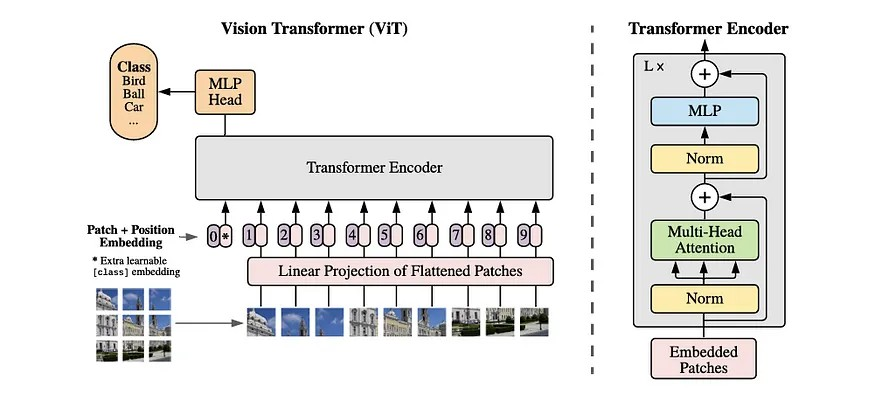
\includegraphics[width=\linewidth]{Figures/ViT.jpg}
  \caption{%
    Overview of the Vision Transformer (ViT) architecture.
    The input image is divided into fixed-size patches, which
    are flattened and projected into a sequence of patch
    embeddings.
    Positional embeddings are added to preserve spatial
    information, and a learnable classification token is
    prepended to the sequence.
    The resulting sequence is processed by a Transformer encoder
    composed of multi-head self-attention and feed-forward
    layers~\cite{dosovitskiy2020vit}.%
  }\label{fig:vit_overview}
\end{figure}


Vision Transformers (ViT) apply the Transformer model,
originally developed for natural language processing, to
computer vision tasks.
Instead of processing images through convolutional filters as in
Convolutional Neural Networks (CNNs), a ViT represents an image
as a sequence of smaller image patches.
The input image is divided into fixed-size patches
(e.g.,~$16 \times 16$ pixels), and each patch is flattened and
projected into a higher-dimensional embedding space.
Positional embeddings are then added to these patch
representations to preserve spatial information, and the
resulting sequence is processed by a Transformer encoder
composed of multi-head self-attention layers and feed-forward
networks, as described in the preceding subsections.

The output of a Vision Transformer is a set of feature
embeddings representing different spatial regions of the image,
each containing high-level semantic information.
However, because the image is divided into relatively large
patches, the resulting feature representation has a
significantly lower spatial resolution than the original input
image.
For a standard ViT with a patch size of $p = 16$, an input
image of size $H \times W$ produces a feature grid of only
$(H/p) \times (W/p)$ embeddings.
While this reduction in resolution improves computational
efficiency and encourages the model to focus on semantically
meaningful patterns, it poses a direct challenge for
dense prediction tasks such as segmentation and depth
estimation, which require high-resolution spatial outputs.
This resolution gap motivates the need for feature upsampling
techniques, discussed in the following section.

\subsection{Vision Foundation Models (VFMs)}

Vision Foundation Models are large-scale neural networks trained
on massive and diverse datasets to produce general-purpose
visual representations.
Unlike traditional task-specific models, foundation models learn
feature representations that transfer to a wide range of
downstream tasks without requiring full retraining.
They typically leverage the Vision Transformer architecture and
produce rich semantic features that capture high-level
information about image content.

Two prominent examples are DINO~\cite{caron2021dino} and CLIP~\cite{radford2021clip}\@.
DINO is a self-supervised learning method that trains Vision
Transformers without requiring labeled data.
It learns meaningful representations by encouraging consistency
between different augmented views of the same image through a
teacher--student training framework, producing features that are
particularly useful for segmentation and object discovery.
CLIP, in contrast, learns visual representations by jointly
training on large-scale image--text pairs using contrastive
learning.
By aligning visual and textual embeddings in a shared
representation space, CLIP can perform zero-shot image
classification and a wide variety of vision-language tasks.
A more recent variant, SigLIP~\cite{zhai2023siglip}, improves on CLIP by replacing
the contrastive loss with a sigmoid-based pairwise loss,
yielding stronger performance particularly at smaller batch
sizes.

Because these models are trained on massive datasets and produce
semantically rich features, they have become the dominant choice
of feature extractor in modern computer vision pipelines.
However, due to their ViT backbone, they all share the same
resolution limitation: their output feature maps are produced at
a fraction of the input resolution, making feature upsampling
an essential post-processing step for any dense prediction task.

%% ============================================================
%%  GROUP 2: Feature Upsampling
%% ============================================================
\section{Feature Upsampling}

\subsection{Interpolation-Based Methods}

Feature upsampling refers to the process of increasing the
spatial resolution of feature maps produced by deep neural
networks.
The simplest approaches rely on classical interpolation
methods, which estimate new values at higher-resolution
coordinates from the surrounding low-resolution features.

\paragraph{Nearest Neighbour Interpolation}
Each upsampled feature is copied from the nearest
low-resolution feature:
\begin{equation}
  F^{HR}(x, y)
  = F^{LR}\!\left(
      \text{round}\!\left(\tfrac{x}{s}\right),\;
      \text{round}\!\left(\tfrac{y}{s}\right)
    \right)
\end{equation}
where $s$ is the upsampling scale factor and $(x, y)$ are
coordinates in the high-resolution map.

\paragraph{Bilinear Interpolation}
Each upsampled feature is a weighted sum of the four nearest
neighbours:
\begin{equation}
  F^{HR}(x, y)
  = \sum_{i=0}^{1} \sum_{j=0}^{1}
    w_{ij}\, F^{LR}(x_i, y_j),
  \qquad
  w_{ij} = (1 - |x - x_i|)(1 - |y - y_j|)
\end{equation}

\paragraph{Bicubic Interpolation}
Bicubic interpolation uses sixteen neighbours and a cubic
kernel:
\begin{equation}
  F^{HR}(x, y)
  = \sum_{i=-1}^{2} \sum_{j=-1}^{2}
    R(i, x)\, R(j, y)\, F^{LR}(x_i, y_j)
\end{equation}
where the cubic kernel is:
\begin{equation}
  R(t) =
  \begin{cases}
    (a+2)|t|^3 - (a+3)|t|^2 + 1, & |t| \le 1 \\
    a|t|^3 - 5a|t|^2 + 8a|t| - 4a, & 1 < |t| < 2 \\
    0, & |t| \ge 2
  \end{cases}
\end{equation}
with $a = -0.5$ for the Catmull-Rom spline.

Although these methods are computationally efficient, they do
not learn how to recover spatial information lost during
downsampling, and they produce blurry or blocky results when
applied to semantic feature maps.
Learnable approaches such as transposed convolution and
sub-pixel convolution (pixel shuffle) address this by training
filters to reconstruct spatial detail from compact feature
representations.
However, all of these approaches remain task-specific and
backbone-specific, requiring retraining or retuning for each new
architecture.
This limitation motivated the development of universal,
coordinate-based upsampling methods, described next.

\subsection{Implicit Neural Representations and LIIF}

Traditional feature representations store information as
discrete grids of fixed resolution.
Implicit Neural Representations (INR) offer an alternative by
representing a signal as a continuous function parameterised by
a neural network.
Given any continuous coordinate as input, the network outputs
the corresponding value at that location, allowing the
representation to be queried at arbitrary resolutions.

Chen et al.\ (2021) applied this principle to image
super-resolution in the Local Implicit Image Function (LIIF).
An encoder produces a low-resolution feature grid from the
input image.
A decoder — implemented as a Multi-Layer Perceptron (MLP) —
then takes a target coordinate and the features of its
surrounding grid cells as input, and outputs the predicted value
at that continuous coordinate.
Because the MLP is a continuous function, the model can
generate outputs at any target resolution during inference,
including resolutions not seen during training.
This coordinate-based formulation became the conceptual
foundation for subsequent universal upsampling models,
including AnyUp.

\subsection{The AnyUp Model}

AnyUp is a state-of-the-art universal feature upsampling model
proposed by Wimmer et al.\ (2025).
Its primary contribution is the ability to upsample feature maps
from any Vision Foundation Model backbone to any target
resolution, without task-specific training or manual tuning for
each backbone.
This backbone-agnostic design is achieved through two key
architectural decisions.

First, a Feature-Agnostic Layer normalises the input feature
maps to remove statistical biases introduced by different
backbone architectures, ensuring that the decoder sees a
consistent input distribution regardless of the feature
extractor used.
Second, a Window Attention module performs the upsampling itself
by treating it as a coordinate-based retrieval problem: for each
target coordinate on the high-resolution grid, a query is formed
from the coordinate embedding and matched against local
low-resolution features using scaled dot-product attention.

AnyUp is trained using a self-supervised strategy that requires
no manual annotations.
Two views of the same image are encoded at different
resolutions; the high-resolution view serves as the
pseudo-ground-truth, and the model is trained to upsample the
low-resolution features to match it using a cosine similarity
loss:
\begin{equation}
  \mathcal{L} = 1 - \cos(\hat{f},\, f)
  \label{eq:anyup_loss}
\end{equation}
where $\hat{f}$ is the predicted high-resolution feature and $f$
is the pseudo-ground-truth.
This loss is backbone-agnostic by design, as cosine similarity
operates on normalised vectors regardless of their origin.

While AnyUp achieves strong results for static images, it
processes video sequences on a frame-by-frame basis, producing
temporally inconsistent outputs due to its complete lack of
inter-frame communication.
This limitation directly motivates the AnyUp3D framework
proposed in this thesis.

\subsection{Window-Based Attention for Upsampling}

Rather than applying attention globally across all spatial
positions — which is computationally prohibitive for
high-resolution feature maps — window-based attention restricts
the attention computation to a local neighbourhood around each
target location.
For a given query position on the high-resolution grid, only
the features within a local window of low-resolution patches
serve as keys and values.
This design dramatically reduces the computational cost of
attention-based upsampling while still providing sufficient
local context to recover fine spatial details.
Window-based attention is the core mechanism of the AnyUp model
and is retained unchanged in the AnyUp3D framework proposed
in this thesis.

%% ============================================================
%%  GROUP 3: Video Understanding and Temporal Modeling
%% ============================================================
\section{Video Understanding and Temporal Modeling}

\subsection{Temporal Consistency}

Temporal consistency refers to the property that visual
representations or predictions remain stable and coherent across
consecutive frames in a video sequence.
When a model processes each frame independently, small
variations in the input features can cause the output to vary
abruptly between adjacent frames, even when the underlying
visual content changes only slightly.
This leads to temporal artifacts such as flickering, jittering
object boundaries, and unstable semantic assignments — all of
which degrade the quality of downstream video understanding
tasks.

Temporal consistency is enforced by encouraging the model to
produce similar representations for temporally adjacent inputs.
This can be achieved through several approaches, including
temporal loss functions that penalise frame-to-frame variation,
motion cues derived from optical flow, and architectures that
explicitly model inter-frame dependencies.
In this work, temporal consistency is addressed architecturally
through the integration of 3D convolutions in the encoder and
3D cross-attention with temporal masking directly into the
upsampling pipeline, as described in Chapter~3.

\subsection{3D Convolution}

3D Convolution is a direct extension of the standard 2D
convolution operation into the temporal dimension.
A 3D convolutional kernel of size $(k \times k \times t)$ slides
simultaneously across the spatial height and width dimensions
and the temporal dimension of a video volume
$(H \times W \times T)$, extracting features that capture both
spatial appearance and temporal motion in a single unified
operation.

This joint spatial-temporal processing is more expressive than
factorised approaches that apply 2D spatial convolutions and 1D
temporal convolutions sequentially, as it can capture
correlations between motion and appearance that would otherwise
be lost.
In the proposed AnyUp3D framework, a 3D convolutional layer
with a kernel of size $3 \times 3 \times 3$ is applied to the
stacked feature volume at the early stage of the decoder, before
spatial upsampling, to extract local spatio-temporal motion
patterns from the input frame window.

\subsection{Temporal Attention}

Temporal Attention is an application of the self-attention
mechanism along the temporal axis of a video sequence.
Rather than computing attention across all spatial positions
within a single frame, temporal attention computes attention
across the same spatial position across multiple frames.
For a given pixel location $(x, y)$ in the current query frame
$t$, a query vector $Q$ is formed from the feature at that
location, while the key matrix $K$ and value matrix $V$ are
constructed from the features at the same location across all
$T$ frames in the temporal window.
The attention score for each frame is computed as the scaled
dot product between the query and the corresponding key,
followed by softmax normalisation:
\begin{equation}
  f_{\text{out}}(x,y,t)
  = \text{softmax}\!\left(
      \frac{Q_{x,y,t}\, K_{x,y,1:T}^{\top}}{\sqrt{d}}
    \right) V_{x,y,1:T}
  \label{eq:temporal_attention}
\end{equation}
The resulting output is a weighted combination of features from
all frames in the window, where frames whose content most
closely resembles the query frame receive the highest attention
weights.
This allows the model to selectively borrow stable evidence from
neighbouring frames to correct inconsistencies in the current
frame, directly suppressing flickering artifacts at the feature
level.

\subsection{Video Object Segmentation (VOS)}

Video Object Segmentation is a computer vision task that
requires identifying and delineating specific objects within
each frame of a video sequence while maintaining consistent
object identity across the full duration of the clip.
The task is typically formulated in a semi-supervised setting,
where the ground-truth segmentation mask of the target object is
provided for the first frame only, and the model must propagate
this mask through all subsequent frames.

VOS is a particularly demanding benchmark for evaluating
temporal consistency because accurate segmentation requires
stable and coherent feature representations across frames.
Any flickering or instability in the underlying feature maps
directly manifests as inconsistent or jittering segmentation
boundaries in the output masks.
For this reason, VOS is used in this work as the primary
downstream evaluation task for the AnyUp3D framework.
Performance is measured using the J\&F metric, which combines
region similarity ($\mathcal{J}$, the Jaccard index) and
contour accuracy ($\mathcal{F}$) into a single score, providing
a comprehensive measure of both spatial accuracy and boundary
sharpness.
The evaluation is conducted on the DAVIS-2017 benchmark, which
provides densely annotated video sequences covering a wide range
of challenging scenarios including fast motion, occlusion, and
appearance change.
\section*{PART II -- LITERATURE REVIEW}
\addcontentsline{toc}{section}{PART II -- LITERATURE REVIEW}

% ── Introduction ─────────────────────────────────────────────
\section{Review of Previous Studies}

The evolution of feature upsampling has transitioned from
rigid, data-independent heuristics to sophisticated,
coordinate-based neural representations.
Over the past decade, this progression has been driven by three
primary research shifts: first, the move from simple spatial
interpolation to content-aware dynamic kernels; second, the
transition from task-specific architectures to universal,
backbone-agnostic frameworks; and third, the ongoing effort to
adapt static image-based models to the temporal demands of
video sequences.

To provide a clear roadmap of this technical trajectory, the
following literature is categorised into three distinct
thematic groups:
\begin{enumerate}
  \item \textbf{Coordinate-Based and Universal Architectures:}
        Focuses on the recent shift toward treating feature maps
        as continuous functions rather than discrete grids,
        enabling arbitrary-scale upsampling across diverse model
        backbones. This group also covers the key Vision
        Foundation Models that serve as the feature extractors
        in these pipelines.

  \item \textbf{Feature Refinement and Structural Denoising:}
        Examines methodologies designed to sharpen semantic
        boundaries and remove artifacts inherent in
        Transformer-based representations.

  \item \textbf{Spatio-Temporal Stability:}
        Explores the specialised techniques developed to
        maintain visual and semantic coherence across dynamic
        video frames, including 3D convolutions, memory-based
        attention, and temporal consistency enforcement.
\end{enumerate}

% ── Group 1 ──────────────────────────────────────────────────
\subsection{Coordinate-Based and Universal Upsampling}

Chen et al.\ (2020) developed the Local Implicit Image
Function (LIIF)~\cite{liif} to overcome the fixed-scale
limitations of discrete image representations in
super-resolution tasks.
By representing images as continuous functions through a
Multi-Layer Perceptron that takes latent codes and target
coordinates as inputs, the research enabled
\textit{infinite resolution scaling}.
The study demonstrated that a single model could generalise to
arbitrary scales not encountered during training, significantly
outperforming traditional interpolation and discrete
upsamplers.
LIIF established the coordinate-based paradigm that underlies
all subsequent universal upsampling models, including those
reviewed below.

Fu et al.\ (2024) introduced FeatUp~\cite{featup}, a
task-and-model-agnostic framework that restores lost spatial
resolution in deep features produced by any Vision Foundation
Model backbone.
The methodology uses a joint bilateral upsampler that fuses
low-resolution semantic features with high-resolution guidance
from the original image through a multi-view consistency loss,
drawing analogies to Neural Radiance Fields (NeRFs).
Two variants are proposed: a fast feedforward upsampler for
general use and an implicit per-image model for arbitrary
resolution.
Crucially, the upsampled features retain their original
semantics and can be directly swapped into existing pipelines
without retraining.
FeatUp demonstrated significant improvements over bilinear
interpolation and task-specific upsamplers across class
activation mapping, segmentation, and depth prediction tasks.
However, like all image-based methods, it processes each
frame independently and produces temporally inconsistent
outputs when applied to video.

Huang et al.\ (2025) introduced LoftUp~\cite{loftup}, a
coordinate-based upsampler designed to extract high-resolution
features from Vision Foundation Models without manual labels.
The methodology utilises a cross-attention transformer to fuse
low-resolution semantic tokens with high-resolution geometric
cues from the original image.
By employing a self-supervised pseudo-ground-truth training
signal derived from class-agnostic masks, the model
successfully recovered fine-grained spatial details --- such as
thin object boundaries --- that are typically lost in
Transformer backbones.
LoftUp advances the field by demonstrating that structural
information from the original image can guide feature
upsampling more precisely than attention alone, though it
remains an image-based method with no temporal modeling
capability.

Wimmer et al.\ (2025) proposed AnyUp~\cite{anyup}, a
state-of-the-art universal upsampler designed to function
across diverse model architectures without task-specific
tuning.
The researchers implemented a feature-agnostic window attention
layer that treats upsampling as a localised re-alignment task,
mapping features from any backbone onto a higher-resolution
grid.
While the model proved superior at preserving semantic
integrity across diverse backbones, the findings highlighted a
critical limitation: its frame-by-frame processing leads to
significant temporal instability in video applications,
producing flickering artifacts at the feature level.
This limitation is the direct motivation for the AnyUp3D
framework proposed in this thesis.

Oquab et al.\ (2024) published DINOv2~\cite{dinov2}, a family
of self-supervised Vision Transformer models trained on a
large curated dataset of 142 million images.
By combining and scaling several pretraining techniques ---
including self-distillation and masked image modelling ---
DINOv2 produces all-purpose visual features that perform
competitively with weakly-supervised models across a wide range
of vision tasks, including segmentation, depth estimation, and
image retrieval, without any fine-tuning.
DINOv2 is directly relevant to this thesis as an example of the
pretrained feature extractors that the backbone-agnostic AnyUp3D
design is compatible with, alongside CLIP and SigLIP\@.
The experiments in Chapter~4 use VideoMAE as the primary feature
extractor; DINOv2, CLIP, and SigLIP represent the broader class
of Vision Foundation Models that AnyUp3D is designed to support
without task-specific retraining.

% ── Group 2 ──────────────────────────────────────────────────
\subsection{Feature Refinement and Structural Denoising}

Wang et al.\ (2019) introduced CARAFE (Content-Aware
ReAssembly of FEatures)~\cite{carafe} to replace standard,
content-blind operators such as bilinear interpolation.
The authors designed a lightweight kernel prediction module
that generates unique upsampling kernels for every spatial
location based on local context, allowing for the
content-aware reassembly of features.
The study proved that adaptive receptive fields significantly
boost performance in object detection and instance
segmentation by following the actual shapes and textures
present in an image.
CARAFE established the importance of content-awareness in
feature upsampling, but its kernels are generated from a
single backbone and cannot be directly applied across
different backbone architectures.

Yang et al.\ (2024) explored the inherent artifacts of Vision
Transformers in their work on Denoising Vision
Transformers~\cite{denoising_vit}.
By identifying that positional embeddings often cause
``checkerboard noise'' in feature maps, they proposed a
two-stage denoising method involving feature decomposition and
a learnable denoiser.
This research established a vital preprocessing step for
cleaning feature maps before upsampling, ensuring that
semantic representations remain sharp and free of structural
interference.
The findings are directly relevant to this project, since the
3D Convolution module in AnyUp3D also receives
positional-embedding-corrupted features from the backbone and
must process them reliably.

% ── Group 3 ──────────────────────────────────────────────────
\subsection{Video and Temporal Consistency}

Cheng et al.\ (2023) presented Cutie~\cite{cutie}, a video
object segmentation network that introduces object-level memory
reading to maintain consistency across frames.
The model utilises a query-based object transformer to
interact with bottom-up pixel features, allowing for
high-level semantic tracking while retaining high-resolution
feature maps.
Their methodology cleanly separated foreground semantics from
background distractors, achieving a significant improvement in
temporal stability on the MOSE dataset compared to previous
pixel-matching baselines.
Although Cutie's memory logic is optimised specifically for
video object segmentation and cannot be easily applied as a
general-purpose upsampler, its object-level temporal memory
mechanism serves as an important conceptual reference for the
temporally-extended 3D cross-attention proposed in this work.

Liu et al.\ (2022) advocated for spatio-temporal locality in
the Video Swin Transformer~\cite{swin}, extending the Swin
architecture to the 3D domain.
By implementing 3D Patch Partitioning and 3D Shifted Window
Attention, the model captures motion characteristics and
spatial relationships simultaneously.
The key finding was that joint spatio-temporal modeling
surpasses factorised models in both efficiency and accuracy,
providing a robust backbone for understanding dynamic video
content through localised 3D kernels.
Video Swin directly validates the design choice of 3D
Convolution in AnyUp3D, demonstrating that jointly
processing spatial and temporal dimensions at the feature
level leads to stronger and more coherent representations
than applying spatial and temporal operations sequentially.

Zhou et al.\ (2024) developed Upscale-A-Video~\cite{upscale_video}
to resolve the flickering artifacts common in AI-generated
video upscaling.
The project integrated 3D Convolutional layers and Temporal
Attention modules into a latent diffusion architecture to
enforce consistency across the time axis.
Their research proved that explicit temporal modeling is
essential for maintaining the coherence of moving textures,
providing a direct blueprint for the temporal extensions
proposed in this thesis.
While Upscale-A-Video is task-specific and computationally
expensive owing to its diffusion backbone, it validates the
combination of 3D convolutions and temporally-extended
cross-attention as the right architectural choices for video
feature stabilisation.

Ravi et al.\ (2024) presented Segment Anything Model 2
(SAM 2)~\cite{sam2}, a foundation model for promptable visual
segmentation in both images and videos.
SAM 2 extends the original Segment Anything Model to the
video domain by introducing a streaming memory attention
module --- a lightweight bank of object-level memories drawn
from previous frames --- that allows the model to track and
segment objects consistently across a full video sequence
in real time.
SAM 2 achieves state-of-the-art results on the DAVIS-2017
benchmark, the same evaluation dataset used in this thesis,
establishing it as the strongest contemporary baseline for
temporally consistent video segmentation.
Crucially, SAM 2's memory mechanism addresses temporal
consistency at the \emph{segmentation mask level}, while
AnyUp3D addresses the same problem at the more
fundamental \emph{feature representation level}, making the
two approaches complementary rather than competing.


% ── Comparative Analysis ─────────────────────────────────────
\section{Comparative Analysis of Previous Work}

The landscape of feature upsampling has evolved through
several technical paradigms: from fixed geometric
interpolation to content-aware dynamic kernels, and finally
toward universal, coordinate-based representations.
The primary challenge currently facing the field is what can
be termed the \textit{Universality-Stability Gap}: models
either provide high backbone flexibility without temporal
coherence, or offer temporal stability at the cost of being
architecture-locked.

The following table evaluates the key studies reviewed above
based on their technical relevance to the development of a
temporally consistent, universal upsampler.

\begin{table}[h!]
\centering
\caption{Technical Comparison of Feature Upsampling and Video
         Consistency Architectures}\label{tab:comparison}
\resizebox{\textwidth}{!}{%
\begin{tabular}{lllll}
\toprule
\textbf{Model}
  & \textbf{Domain}
  & \textbf{Backbone Compatibility}
  & \textbf{Core Strengths}
  & \textbf{Technical Weaknesses} \\
\midrule
LIIF~\cite{liif}
  & Image
  & Backbone-Agnostic
  & Infinite resolution scaling
  & Limited to RGB\@; ignores deep semantics \\
CARAFE~\cite{carafe}
  & Image
  & Task-Specific
  & Content-aware reassembly
  & Requires manual backbone tuning \\
FeatUp~\cite{featup}
  & Image
  & \textbf{Backbone-Agnostic}
  & High-res features, any backbone
  & Frame-independent; temporal jitter \\
LoftUp~\cite{loftup}
  & Image
  & Backbone-Agnostic
  & Sharpens VFM boundaries
  & No temporal modeling \\
AnyUp~\cite{anyup}
  & Image
  & \textbf{Backbone-Agnostic}
  & State-of-the-art semantic retention
  & \textbf{Zero temporal context for video} \\
Video Swin~\cite{swin}
  & Video
  & Architecture-Locked
  & Local 3D temporal context
  & Incompatible with external FM features \\
Upscale-A-Video~\cite{upscale_video}
  & Video
  & Task-Specific
  & High visual fidelity via 3D Conv
  & High compute; restricted to diffusion \\
Cutie~\cite{cutie}
  & Video
  & Task-Specific
  & Long-range object memory
  & Optimised only for segmentation masks \\
SAM 2~\cite{sam2}
  & Video
  & Task-Specific
  & Streaming memory; SOTA on DAVIS
  & Mask-level only; no feature upsampling \\
\textbf{AnyUp3D (Ours)}
  & \textbf{Video}
  & \textbf{Backbone-Agnostic}
  & \textbf{Universal + temporal consistency}
  & \textbf{Increased spatio-temporal complexity} \\
\bottomrule
\end{tabular}%
}
\end{table}

\begin{center}
  \textbf{Synthesis of Technical Relevance}
\end{center}

This comparative study highlights a critical structural void
in current upsampling methodologies.
Early learned approaches such as \textit{CARAFE} established
the superiority of content-aware upsampling over bilinear
methods but lacked the backbone compatibility required for the
diverse ecosystem of modern Vision Foundation Models.
This was addressed by coordinate-based systems such as
\textit{LIIF}, \textit{FeatUp}, and \textit{AnyUp}, which
treat feature maps as continuous functions and operate across
any backbone architecture.
While these models excel in modularity and semantic fidelity,
their independent frame processing makes them technically
insufficient for video, producing spatially accurate but
temporally disjointed features that manifest as flickering.

In contrast, dedicated video architectures such as
\textit{Video Swin}, \textit{Cutie}, and \textit{SAM 2}
provide the necessary infrastructure for temporal stability.
\textit{Video Swin} captures local motion through 3D kernels,
\textit{Cutie} introduces object-level memory reading, and
\textit{SAM 2} brings real-time streaming memory attention
for consistent video segmentation.
However, these models are fundamentally task-specific or
architecture-locked and cannot be applied as general-purpose
feature upsamplers for arbitrary backbones such as DINOv2 or
CLIP\@.

\textit{AnyUp3D} is architected to unify these two
paradigms.
By incorporating the 3D convolutional spatial-temporal modeling
of \textit{Video Swin} and the temporal attention mechanism of
\textit{Upscale-A-Video} into the backbone-agnostic framework
of \textit{AnyUp} --- realised as 3D cross-attention with
temporal masking --- we resolve the flickering artifacts found
in existing universal baselines.
This approach provides a first-of-its-kind solution that
maintains the flexibility of a Foundation Model upsampler
while enforcing the rigorous inter-frame consistency required
for high-resolution video understanding.


% ── Research Gap ─────────────────────────────────────────────
\section{Research Gap and Project Contribution}

The literature review reveals a clear dichotomy:
\begin{itemize}
  \item \textbf{Universal Upsamplers} (FeatUp, LoftUp, AnyUp)
        provide flexibility across tasks and backbones but fail
        to handle the temporal dimension, leading to
        inconsistent and flickering results in video.
  \item \textbf{Video Consistency Models}
        (Upscale-A-Video, SAM 2, Cutie) provide stability but
        are designed for specific tasks and cannot be easily
        applied as general feature upsamplers across arbitrary
        Vision Foundation Model backbones.
\end{itemize}

\textbf{Project Contribution:}
This project addresses this gap by proposing
\textit{AnyUp3D}.
We contribute a novel architecture that integrates the
\emph{temporal stability} mechanisms of video models ---
specifically 3D convolutions in the encoder (validated by
\textit{Video Swin}) and 3D cross-attention with temporal masking
(validated by \textit{Upscale-A-Video}) --- into the
\emph{universal framework} of AnyUp.
This yields the first task-agnostic, backbone-agnostic feature
upsampler capable of producing temporally consistent results
for video sequences.




 % Lit Review
% chktex-file 13 24
\chapter{METHODOLOGY}

\section{Chapter Overview}
This chapter presents the engineering methodology followed to design, implement, and
evaluate the proposed AnyUp3D framework. AnyUp~\cite{anyup} addresses the low-resolution
feature map limitation of Vision Foundation Models (VFMs) such as DINOv2~\cite{dinov2} and CLIP~\cite{radford2021clip}
by enabling continuous, backbone-agnostic spatial upsampling. However, when applied
to video, AnyUp~\cite{anyup} processes each frame independently, ignoring inter-frame correlations
and producing flickering artifacts and unstable object boundaries. AnyUp3D extends
AnyUp~\cite{anyup} into the temporal domain by integrating two novel components into its upsampling
pipeline: \textbf{3D convolutions} inside the encoder to capture spatiotemporal patterns across
adjacent frames, and \textbf{3D cross-attention with temporal masking} to correct frame-level
inconsistencies by attending to neighboring frames within a spatiotemporal window. These additions introduce temporal
consistency while preserving the backbone-agnostic universality that defines the
original AnyUp~\cite{anyup} design.

The chapter is organized into the following stages:
\begin{enumerate}
    \item \textbf{Requirements and Specifications}, defining the functional and
    performance criteria the system must meet;
    \item \textbf{Possible Scenarios}, justifying the chosen architectural approach
    over alternatives;
    \item \textbf{System Framework}, presenting the overall three-stage pipeline and
    data flow, highlighting the novel temporal contributions;
    \item \textbf{Dataset Description}, documenting the UCF-101 training dataset
    and the DAVIS-2017 evaluation benchmark;
    \item \textbf{Implementation Details}, explaining how the model was constructed
    and integrated; and
    \item \textbf{Evaluation Plan}, defining the loss-based proxy metrics and
    held-out validation strategy used to monitor and validate the system's performance.
\end{enumerate}

Each stage is presented with a clear justification of the engineering decisions made
to ensure temporal consistency while preserving the universality and
backbone-agnostic nature of the original AnyUp~\cite{anyup} design.

\section{Requirements and Specifications}
Based on the problem analysis presented in Chapter One, the following requirements were identified for the proposed AnyUp3D system.

\subsection{Functional Requirements}
\begin{itemize}
    \item The system must accept a sequence of consecutive video frames alongside their 
    corresponding low-resolution feature maps as input, and produce temporally consistent, 
    high-resolution feature maps as output.
    \item The system must support arbitrary upsampling scales, preserving the resolution-agnostic behavior of the original AnyUp~\cite{anyup} model.
    \item The system must reduce temporal inconsistency artifacts (flickering, jittering object boundaries) compared to the frame-by-frame AnyUp~\cite{anyup} baseline, as measured by the mean cosine similarity between adjacent predicted frames on the DAVIS-2017 validation sequences.
    \item The system must maintain competitive spatial accuracy, measured by the J\&F score on DAVIS-2017, relative to the original AnyUp~\cite{anyup} baseline.

\end{itemize}

\subsection{Non-Functional Requirements}
\begin{itemize}
    \item \textbf{Backbone Agnosticism:} The temporal modules must integrate into the AnyUp~\cite{anyup} pipeline without making any assumptions about the feature extractor used.
    \item \textbf{Scalability:} The model must be trainable on available academic GPU hardware, with the sequence length $T$ and batch size serving as adjustable parameters to accommodate memory constraints.
    \item \textbf{Scope Constraints:} Real-time processing is explicitly out of scope for this project; the primary focus is on accuracy and temporal stability rather than inference speed.
\end{itemize}

\section{Possible Scenarios}

This section documents three concrete design decisions encountered during the 
development of AnyUp3D, the alternatives considered for each, and the 
justification for the choice made.

%-----------------------------------------------------------
\subsection{Training: How to Supervise the Upsampler}

Training a feature upsampler requires a source of high-quality supervision.
Computing teacher features from arbitrarily high-resolution inputs is
computationally infeasible at scale and moves most vision backbones
out of distribution. Two practical training strategies from the literature
were considered:

\begin{itemize}
    \item \textbf{Option A --- JAFAR strategy~\cite{couairon2025}:} Train entirely
    at low resolutions, where both the supervision signal and the student input are
    derived from the same input frames without an engineered resolution gap.
    Couairon et al.\ argue that low-resolution training is sufficient for learning
    a generalisable attention-based upsampling mechanism.
    \item \textbf{Option B --- AnyUp crop-based strategy~\cite{anyup}:} Sample a
    high-resolution spatial crop from the input and pass it to the frozen teacher
    to obtain the feature targets. Simultaneously downsample the same crop to
    produce a lower-resolution student input. The upsampler learns to recover the
    teacher's features across this explicit resolution gap.
\end{itemize}

\paragraph{Decision: Option B was adopted.}
The AnyUp~\cite{anyup} crop-based strategy was selected because it provides a true
high-resolution supervision signal: the teacher's feature targets are extracted from
a 224-pixel crop, while the student input is derived from a 112-pixel downsampled
version of the same crop, giving the model a non-trivial upsampling objective.
This resolution gap forces the upsampler to learn genuine spatial recovery rather
than approximate low-resolution feature interpolation. For video, the crop is applied
as a consistent spatial tube across all $T$ frames, ensuring that the teacher and
student always observe the same scene region and that the temporal supervision signal
remains coherent across the clip.

%-----------------------------------------------------------
\subsection{Training: How to Sample Frames from a Video Clip}

The temporal sampling interval determines how much real-world motion separates
consecutive sampled frames. Too small an interval produces near-identical frames
that trivialise the temporal consistency objective; too large an interval produces
clips that no longer represent coherent temporal sequences. When constructing a
training clip of $T$ frames from a raw video, two strategies were considered:

\begin{itemize}
    \item \textbf{Option A --- Dense sampling (every $k$ frames):} Select $T$ 
    consecutive frames with a fixed stride $k$ regardless of the video's frame 
    rate.
    \item \textbf{Option B --- Time-based sampling (one frame per $t$ seconds):} 
    Select frames at fixed temporal intervals measured in wall-clock time, so 
    that the sampled clip covers the same real-world duration regardless of the 
    video's frame rate.
\end{itemize}

\paragraph{Decision: Option B was adopted, with $t = 0.5$ seconds (2 frames per second).}
Dense sampling on high frame-rate video produces near-identical consecutive frames,
making the temporal consistency objective trivially easy and non-generalisable. A
fixed frame stride applied to low-frame-rate video skips too much visual content,
distorting the motion dynamics of the clip. Anchoring the interval to $t = 0.5$
seconds of wall-clock time maintains a consistent real-world tempo regardless of
the source frame rate, giving the temporal modules a meaningful and uniform learning
signal throughout training.

%-----------------------------------------------------------
\subsection{Architecture: How to Extend the Windowed Attention to the Temporal 
Domain}

The spatial upsampling core of AnyUp~\cite{anyup} relies on windowed cross-attention, in which 
each high-resolution query token attends only to key tokens within a local spatial 
window in the low-resolution feature map. Extending this mechanism to video 
required a decision on how to incorporate the temporal dimension into the attention 
receptive field. Three options were considered:

\begin{itemize}
    \item \textbf{Option 1 --- 3D attention window:} Extend the existing spatial 
    window with an additional temporal axis, so each query token attends to 
    spatially nearby key tokens within a fixed number of neighboring frames.
    \item \textbf{Option 2 --- 2D spatial window with global temporal attention:} 
    Keep the spatial window unchanged but allow each query to attend to all 
    frames simultaneously, removing any temporal locality constraint.
    \item \textbf{Option 3 --- Separate spatial and temporal attention modules:} 
    Retain the original 2D windowed attention for spatial upsampling and add a 
    dedicated second attention module that operates purely along the temporal 
    axis.
\end{itemize}

\paragraph{Decision: Option 1 was adopted.}
Option 2 introduces quadratic scaling in the temporal dimension: removing the 
temporal locality constraint multiplies the size of the attention matrix by $T$, 
making it prohibitively memory-expensive at moderate resolutions and frame counts. 
Option 3 avoids this cost but introduces architectural redundancy: two separate 
attention mechanisms must be trained and maintained, their combined parameters 
increase the model's footprint, and the interaction between spatial and temporal 
signals is factorised rather than jointly modelled. The 3D window approach of 
Option 1 addresses both concerns simultaneously. Temporal locality bounds the 
attention matrix to a fixed size regardless of clip length, and joint 
spatiotemporal attention allows the model to reason about spatial detail and 
temporal context within a single unified operation. It is also the most 
conservative extension of the existing windowed attention: only the mask 
computation changes, while the attention layer itself remains unchanged.

%-----------------------------------------------------------
\subsection{Architecture: Temporal Window Parameterization --- Ratio or Frame 
Count?}

Having decided to use a 3D attention window, a secondary decision arose regarding 
how to parameterize the size of the temporal window. Two representations were 
considered:

\begin{itemize}
    \item \textbf{Option A --- Temporal ratio:} Express the temporal window as a 
    fraction of the total clip length $T$, so the number of attended neighboring 
    frames scales proportionally as $T$ changes.
    \item \textbf{Option B --- Absolute frame count:} Express the temporal window 
    as a fixed number of neighboring frames $w_t$, independent of the total clip 
    length.
\end{itemize}

\paragraph{Decision: Option B was adopted, with $w_t = 4$.}
A ratio-based window scales with $T$: a window of $0.5$ covers 4 frames for a 
clip of $T = 8$ but 8 frames for a clip of $T = 16$. This causes the model's 
effective temporal receptive field to change as $T$ grows through the curriculum, 
making the behaviour of the temporal attention inconsistent across training stages. 
More critically, for long videos with many frames, a fixed ratio forces each query 
to attend to a large and growing number of temporally distant frames, inflating 
both the attention matrix and the gradient signal with content that is not 
temporally relevant to the current frame. An absolute frame count $w_t = 4$ keeps 
the temporal receptive field constant regardless of clip length, ensuring that the 
model learns a consistent and transferable notion of neighboring context --- from 
the short clips used in early curriculum stages, to longer clips used later, and 
to arbitrarily long videos at inference time.

\section{System Framework}

\begin{figure}[htbp]
\centering
\resizebox{\textwidth}{!}{%
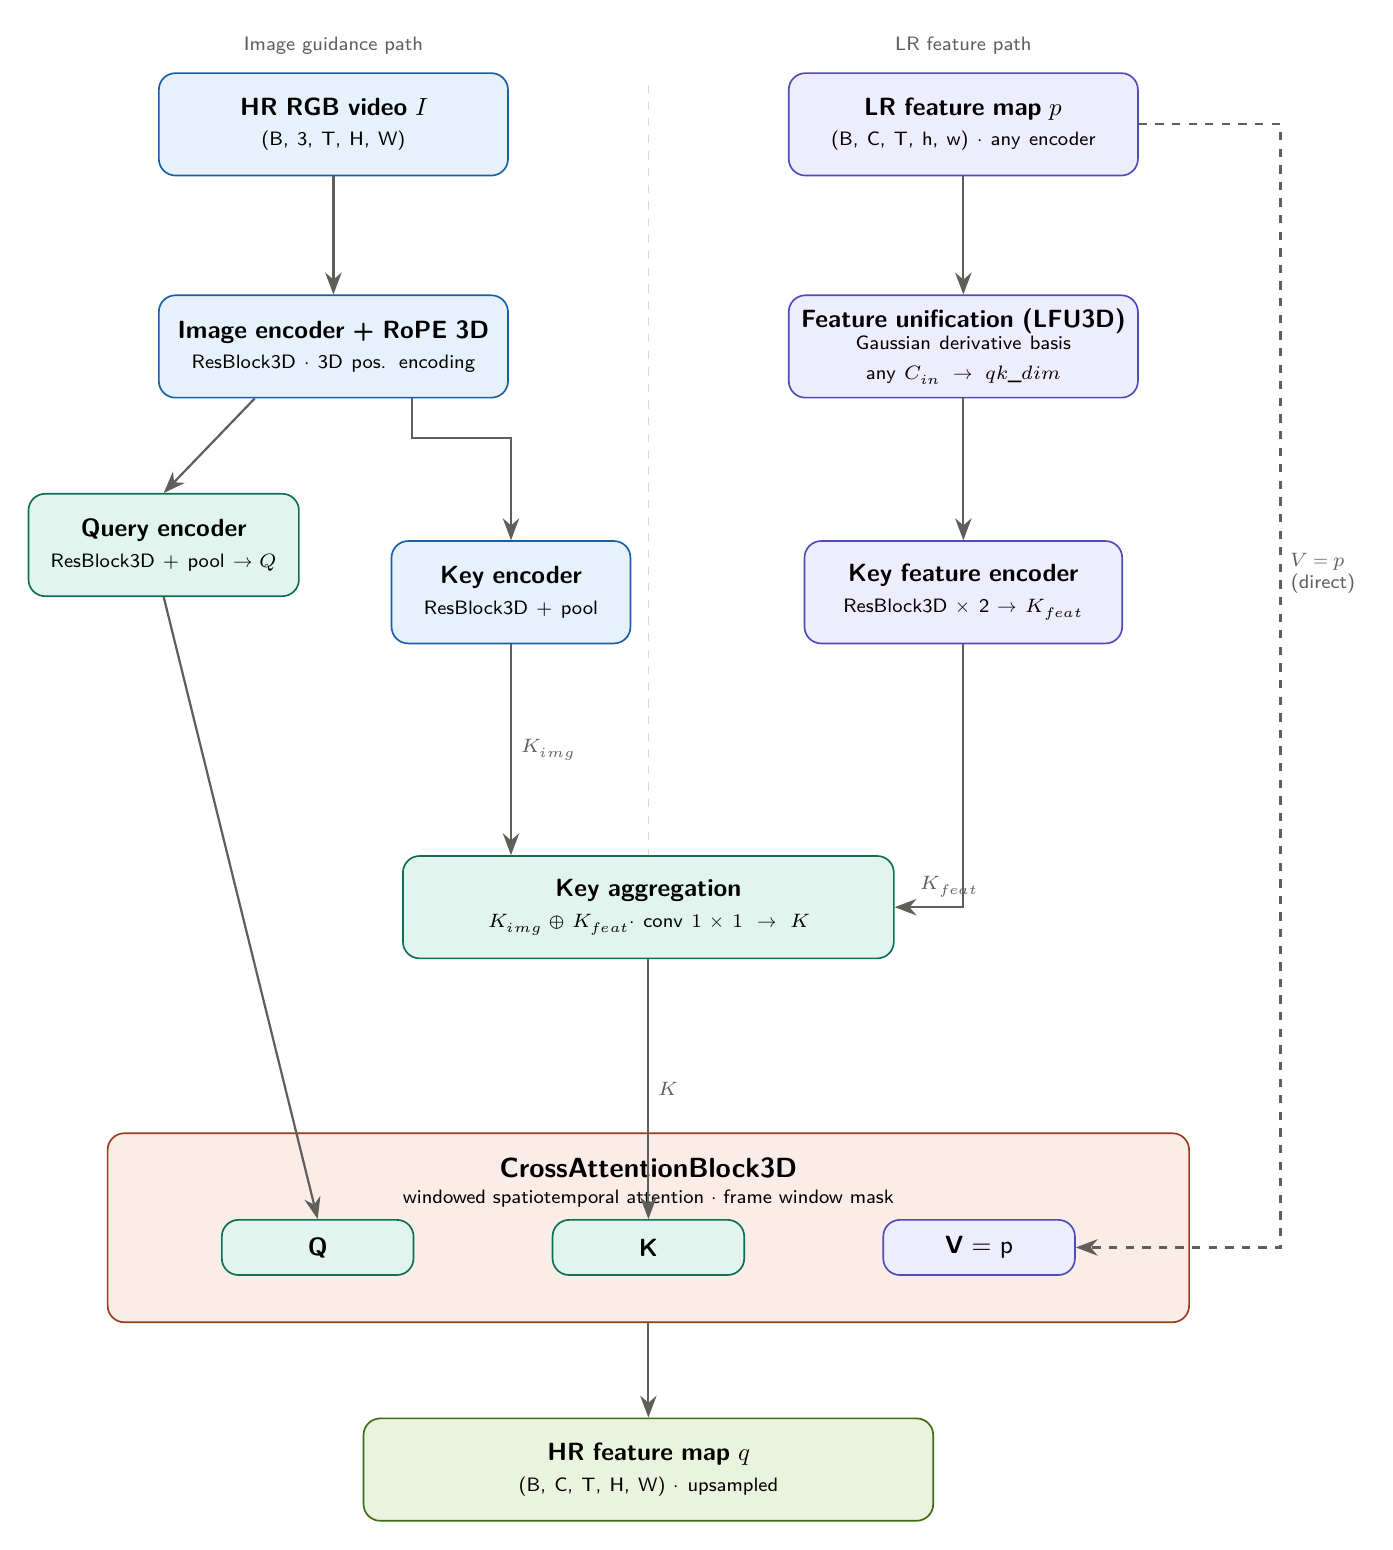
\begin{tikzpicture}[
    node distance=1.2cm and 0.8cm,
    font=\sffamily\small,
    box/.style={
        rectangle, rounded corners=6pt, draw, line width=0.6pt,
        text width=4.2cm, minimum height=1.3cm, align=center
    },
    blueBox/.style={box, fill=blue50, draw=blue600},
    purpleBox/.style={box, fill=purple50, draw=purple600},
    tealBox/.style={box, fill=teal50, draw=teal600},
    coralBox/.style={box, fill=coral50, draw=coral600, text width=13.5cm, minimum height=2.4cm},
    greenBox/.style={box, fill=green50, draw=green600, text width=7cm},
    subBox/.style={box, minimum height=0.7cm, text width=2.2cm},
    arrow/.style={-{Stealth[scale=1.2]}, thick, draw=gray600},
    label/.style={font=\sffamily\scriptsize, text=gray600}
]

    \definecolor{blue50}{HTML}{E6F1FB}
    \definecolor{blue600}{HTML}{185FA5}
    \definecolor{purple50}{HTML}{EEEDFE}
    \definecolor{purple600}{HTML}{534AB7}
    \definecolor{teal50}{HTML}{E1F5EE}
    \definecolor{teal600}{HTML}{0F6E56}
    \definecolor{coral50}{HTML}{FAECE7}
    \definecolor{coral600}{HTML}{993C1D}
    \definecolor{green50}{HTML}{EAF3DE}
    \definecolor{green600}{HTML}{3B6D11}
    \definecolor{gray600}{HTML}{5F5E5A}

    \node[label] (imgLabel) at (0, 1.0) {Image guidance path};
    \node[label] (featLabel) at (8, 1.0) {LR feature path};
    \draw[dashed, color=gray!30] (4, 0.5) -- (4, -11.5);

    \node[blueBox] (hr_input) at (0,0) {
        \textbf{HR RGB video $I$} \\
        \scriptsize (B, 3, T, H, W)
    };

    \node[purpleBox] (lr_input) at (8,0) {
        \textbf{LR feature map $p$} \\
        \scriptsize (B, C, T, h, w) $\cdot$ any encoder
    };

    \node[blueBox, below=1.5cm of hr_input] (img_enc) {
        \textbf{Image encoder + RoPE 3D} \\
        \scriptsize ResBlock3D $\cdot$ 3D pos. encoding
    };

    \node[purpleBox, below=1.5cm of lr_input] (lfu3d) {
        \textbf{Feature unification (LFU3D)} \\
        \scriptsize Gaussian derivative basis \\
        \scriptsize any $C_{in} \to qk\_dim$
    };

    \node[tealBox, below left=1.2cm and -1.8cm of img_enc, text width=3.2cm] (q_enc) {
        \textbf{Query encoder} \\
        \scriptsize ResBlock3D + pool $\to Q$
    };

    \node[blueBox, below right=1.8cm and -1.5cm of img_enc, text width=2.8cm] (k_img_enc) {
        \textbf{Key encoder} \\
        \scriptsize ResBlock3D + pool
    };

    \node[purpleBox, below=1.8cm of lfu3d, text width=3.8cm] (k_feat_enc) {
        \textbf{Key feature encoder} \\
        \scriptsize ResBlock3D $\times$ 2 $\to K_{feat}$
    };

    \node[tealBox, below=5.8cm of img_enc, xshift=4cm, text width=6cm] (k_agg) {
        \textbf{Key aggregation} \\
        \scriptsize $K_{img} \oplus K_{feat} \cdot$ conv $1\times1 \to K$
    };

    \node[coralBox, below=2.2cm of k_agg] (attn_block) {};
    \node[anchor=north, font=\sffamily\bfseries, yshift=-0.2cm] at (attn_block.north) {CrossAttentionBlock3D};
    \node[anchor=north, font=\sffamily\scriptsize, yshift=-0.6cm] at (attn_block.north) {windowed spatiotemporal attention $\cdot$ frame window mask};

    \node[tealBox, subBox, below=1.1cm of attn_block.north, xshift=-4.2cm] (q_node) {\textbf{Q}};
    \node[tealBox, subBox, below=1.1cm of attn_block.north, xshift=0cm] (k_node) {\textbf{K}};
    \node[purpleBox, subBox, below=1.1cm of attn_block.north, xshift=4.2cm] (v_node) {\textbf{V} = p};

    \node[greenBox, below=1.2cm of attn_block] (output) {
        \textbf{HR feature map $q$} \\
        \scriptsize (B, C, T, H, W) $\cdot$ upsampled
    };

    \draw[arrow] (hr_input.south) -- (img_enc.north);
    \draw[arrow] (lr_input.south) -- (lfu3d.north);

    \draw[arrow] ($(img_enc.south)+(-1,0)$) -- (q_enc.north);
    \draw[arrow] (q_enc.south) -- (q_node.north);

    \draw[arrow] ($(img_enc.south)+(1,0)$) -- ($(img_enc.south)+(1,-0.5)$) -| (k_img_enc.north);
    \draw[arrow] (k_img_enc.south) -- (k_img_enc.south |- k_agg.north) node[midway, right, label] {$K_{img}$};

    \draw[arrow] (lfu3d.south) -- (k_feat_enc.north);
    \draw[arrow] (k_feat_enc.south) |- (k_agg.east) node[pos=0.6, above, label] {$K_{feat}$};

    \draw[arrow] (k_agg.south) -- (k_node.north) node[midway, right, label] {$K$};

    \draw[arrow, dashed] (lr_input.east) -- ++(1.8,0) |- (v_node.east) node[pos=0.2, right, label, align=left] {$V=p$\\ (direct)};

    \draw[arrow] (attn_block.south) -- (output.north);

\end{tikzpicture}%
}
\caption{System framework of the proposed AnyUp3D pipeline, showing the image-guidance path, low-resolution feature path, key aggregation, and the final cross-attention-based upsampling block.}
\label{fig:anyup3d_framework}
\end{figure}

\subsection{Stage 1: Input Volume Construction}

AnyUp3D takes two input streams. The first is a \textbf{high-resolution (HR) RGB video} $I \in \mathbb{R}^{B \times 3 \times T \times H \times W}$, which supplies the fine-grained structural and temporal guidance needed for high-fidelity upsampling. It is processed by stacked 3D Residual Blocks (Section~\ref{sec:resblock3d}) followed by \textbf{3D Rotary Positional Encoding (RoPE3D)} (Section~\ref{sec:rope3d}), which injects relative spatiotemporal position into the token representations by rotating query and key vectors according to their $(t, h, w)$ coordinates.

The second input is a \textbf{low-resolution (LR) feature map} $p \in \mathbb{R}^{B \times C \times T \times h \times w}$. Rather than utilizing static image encoders, this volume is extracted from a frozen, pre-trained \textbf{video processing backbone} such as \textbf{VideoMAE} or \textbf{Video Swin Transformer}. These backbones are uniquely suited to produce feature maps that encapsulate deep semantic information across both spatial and temporal dimensions. Within the AnyUp3D pipeline, these features are passed through a \textbf{Feature Unification (LFU3D)} module (Section~\ref{sec:lfu3d}), which employs a learned basis to map arbitrary input channel dimensions to a unified internal representation ($qk\_dim$). While the HR video generates the Queries ($Q$) and a portion of the Keys ($K_{img}$), the LR feature map serves both as a source for the key-feature encoding ($K_{feat}$) and directly as the Value ($V$) component for the subsequent cross-attention mechanism. All backbone weights are kept frozen throughout training to preserve the backbone-agnostic property of the system.

\subsection{Stage 2: Spatiotemporal Feature Encoding}

Once the input volumes are constructed, the system processes the image guidance and the low-resolution latent features through specialized encoding paths to prepare the Query ($Q$), Key ($K$), and Value ($V$) tensors for cross-attention.

\subsubsection{Guidance Path and 3D Rotary Positional Encoding}
The high-resolution guidance video $I$ is first processed by a series of 3D Residual Blocks (\textit{ResBlock3D}), which utilize 3D convolutions to extract local spatiotemporal features. To ensure the model is aware of the global spatiotemporal structure, we apply \textbf{3D Rotary Positional Encoding (RoPE3D)}. Unlike standard additive positional embeddings, RoPE3D operates by applying a rotation transformation to the feature tokens based on their 3D coordinates $(t, h, w)$. 

Specifically, for a feature vector $x$ at a given coordinate, the transformation is defined as:
\begin{equation}
    \text{RoPE3D}(x, \text{coords}) = x \cos(\Theta) + \text{rotate\_half}(x) \sin(\Theta)
\end{equation}
where $\Theta$ is the product of the coordinates and a learned frequency matrix. This approach preserves relative distances between tokens across both space and time, allowing the subsequent attention mechanism to leverage precise geometric and temporal relationships.

\subsubsection{Latent Path and Learned Feature Unification (LFU3D)}
To maintain a backbone-agnostic architecture, the system must handle latent features $p$ from various video encoders with differing channel dimensions. This is achieved through the \textbf{Learned Feature Unification (LFU3D)} module. The LFU3D module employs a depthwise 3D convolution with a learned basis $\mathcal{B} \in \mathbb{R}^{C_{out} \times 1 \times t_k \times k \times k}$. 

The module computes an attention-weighted average across the input channels:
\begin{equation}
    \text{LFU3D}(p) = \text{mean}_{C} \left( \text{Softmax}(\text{Conv3D}_{depth}(p, \mathcal{B})) \right)
\end{equation}
This operation ensures that the output is invariant to the input channel dimensionality of the backbone, effectively mapping arbitrary features into a unified $qk\_dim$ space. The unified features are then passed through a key feature encoder to form $K_{feat}$, which is subsequently fused with the image-based keys $K_{img}$ through a concatenation and $1 \times 1$ convolution to produce the final Key tensor $K$.
\subsection{Stage 3: Spatiotemporal Cross-Attention and Upsampling}

The final stage of the AnyUp3D pipeline performs the localized fusion of high-resolution structural cues and low-resolution semantic features. This is achieved through \texttt{CrossAttentionBlock3D} (Section~\ref{sec:crossattn3d}), a windowed spatiotemporal cross-attention mechanism that ensures both spatial detail and temporal consistency in the upsampled output.

\subsubsection{Query, Key, and Value Preparation}
Before entering the attention mechanism, the encoded representations are projected into a unified embedding space:
\begin{itemize}
    \item \textbf{Queries ($Q$):} The guidance features are passed through the \textit{query\_encoder} and upsampled to the target high-resolution $(H, W)$ using adaptive 3D average pooling. To smooth the upsampled guidance signal and prevent grid artifacts, a $1 \times 3 \times 3$ spatial convolution is applied within the attention block.
    \item \textbf{Keys ($K$):} The model constructs a composite Key by concatenating image-based keys ($K_{img}$) with encoded feature keys derived from the normalized latent volume. These are fused via a \textit{Key Aggregation} layer using a $3 \times 3 \times 3$ convolution, ensuring the Key tensor contains both semantic and structural context.
    \item \textbf{Values ($V$):} Following a direct bypass design, the original low-resolution feature map $p$ is used as the Value tensor. This preserves the integrity of the backbone's latent representations without additional transformation.
\end{itemize}

\subsubsection{Windowed Spatiotemporal Attention Masking}
To manage the quadratic computational complexity of 3D attention, AnyUp3D employs a constrained attention mask. The receptive field of each high-resolution query token is restricted to a 3D local window within the key-value space.

The mask $\mathcal{M}$ is defined by two constraints:
\begin{enumerate}
    \item \textbf{Spatial Constraint:} A spatial window ratio $\alpha$ defines a radius around the projected coordinates of the query. A query at $(h_q, w_q)$ can only attend to keys within the spatial bounds defined by $\pm \alpha$.
    \item \textbf{Temporal Constraint:} The temporal window $w_t$ restricts attention to neighboring frames. A query at frame $t_q$ only attends to keys at frames $t_k$ where $|t_q - t_k| \leq w_t$.
\end{enumerate}
The resulting boolean mask $\mathcal{M} \in \{0, 1\}^{T H W \times T h w}$ is applied to the attention scores, forcing the model to aggregate features from a logically relevant spatiotemporal neighborhood.

\subsubsection{Feature Fusion and Final Output}
The cross-attention operation uses the prepared $Q, K, V$ and the 3D mask to compute the upsampled feature map $q \in \mathbb{R}^{B \times C \times T \times H \times W}$. By normalizing the queries and keys using \textit{RMSNorm} and employing multi-head attention, the model effectively ``paints'' the deep semantic values onto the high-resolution guidance grid. 

Notably, the implementation ensures that if $T=1$ and $w_t=0$, the 3D temporal logic collapses, making the system mathematically equivalent to the 2D AnyUp~\cite{anyup} baseline. This maintains backward compatibility with image-based backbones while enabling state-of-the-art spatiotemporal upsampling for video-based encoders.

\section{Dataset Description}
This section describes the datasets utilized to develop and evaluate the performance of the proposed AnyUp3D system. To ensure the model achieves both spatiotemporal robustness and high-fidelity reconstruction, a dual-dataset strategy was adopted: the \textbf{UCF-101} dataset was used for training, while the \textbf{DAVIS-2017} benchmark served as the primary evaluation set.

\subsection*{Training Dataset: UCF-101 (Action Recognition Data)}
\begin{itemize}
    \item \textbf{Data Type:} RGB video clips sourced from YouTube, categorized into 101 distinct action classes.
    \item \textbf{Source:} Soomro et al.~\cite{soomro2012ucf101} (2012). It is a widely cited benchmark in the video understanding and computer vision communities.
    \item \textbf{Data Description:} The dataset comprises 13,320 video sequences featuring 101 action categories, such as sports, human-object interaction, and body motions. These clips are characterized by unconstrained environments, varying camera motion, background clutter, and diverse lighting conditions. For this work, training is conducted on a subset restricted to the ten most frequent action classes (approximately 1,170 training and 460 test clips), chosen for manageable size and diversity of motion types.
    \item \textbf{Relevance to This Work:} UCF-101 is selected for the training phase because its immense diversity in motion patterns and real-world ``noisy'' footage forces the feature upsampler to learn generalized representations. By training on a wide array of temporal dynamics, the AnyUp3D system becomes robust to unpredictable object movements and camera shakes, which is essential for general-purpose feature upsampling.
\end{itemize}

\subsection*{Evaluation Dataset: DAVIS-2017 (Densely Annotated Video Segmentation)}
\begin{itemize}
    \item \textbf{Data Type:} High-resolution (1080p) RGB video sequences with dense, per-frame, per-object segmentation masks for multiple objects per scene.
    \item \textbf{Source:} Pont-Tuset et al.\ (2017), available at the official DAVIS benchmark website (\url{https://davischallenge.org}). 
    \item \textbf{Data Description:} The dataset contains 150 sequences divided into training, validation, and test-dev splits. Each sequence captures a distinct real-world scene featuring complex challenges, including fast motion, motion blur, occlusion, and scale variation. This work utilizes the validation split (30 sequences, $\sim$2,023 frames) for evaluation.
    \item \textbf{Relevance to This Work:} While UCF-101 provides the breadth required for training, DAVIS-2017 provides a rigorous evaluation setting. Its properties support two complementary assessments:
    \begin{enumerate}
        \item \textbf{Spatial Fidelity:} The dense per-frame segmentation masks enable precise measurement of region similarity ($\mathcal{J}$ score) and contour accuracy ($\mathcal{F}$ score).
        \item \textbf{Temporal Stability:} The DAVIS-2017 sequences provide a diverse set of real-world video clips across which the temporal stability of upsampled features can be assessed via mean cosine similarity between adjacent predicted frames. This metric operates on the model's own predictions and does not use the DAVIS annotations.
        \item \textbf{Fair Comparison:} As the standard benchmark for related architectures such as Cutie and Video Swin Transformer, it enables direct and transparent performance comparison.
    \end{enumerate}
\end{itemize}

\section{Implementation Details}

The proposed system is implemented entirely in Python, using PyTorch as the deep learning framework. The model is designed to operate on five-dimensional tensors of shape $(B, C, T, H, W)$, representing a batch of $B$ video clips each containing $T$ frames of spatial resolution $H \times W$ with $C$ channels. The overall architecture, referred to as AnyUp3D, extends the pretrained 2D AnyUp model \cite{anyup} into the spatiotemporal domain by introducing a temporal axis across all major computational components, including convolutional layers, positional encodings, and the cross-attention mechanism. A frozen VideoMAE encoder \cite{videomae}, based on a Vision Transformer (ViT-B) pretrained on video data, serves as the teacher model, providing dense spatiotemporal feature targets of shape $(B, 768, T', H', W')$ that supervise the training of AnyUp3D.

The implementation is organized into a set of independent modules, each responsible for a specific component of the architecture. The following subsections describe these modules in order, beginning with the spatiotemporal positional encoding mechanism.

%-----------------------------------------------------------
\subsection{Positional Encoding}
\label{sec:rope3d}

Positional information is a critical component in attention-based architectures, as the self- and cross-attention operations are inherently permutation-invariant and carry no built-in notion of spatial or temporal location. The original AnyUp~\cite{anyup} model employs a two-dimensional Rotary Position Embedding (RoPE) \cite{su2024rope} to encode the $(x, y)$ spatial coordinates of each token before they enter the cross-attention module. RoPE encodes position by rotating query and key vectors in the embedding space by an angle that is a function of both the token position and the frequency assigned to each embedding dimension, which allows the dot-product attention scores to depend on the \emph{relative} positions of token pairs rather than their absolute coordinates. To support video inputs, this encoding is extended to three axes: temporal ($z$), horizontal spatial ($x$), and vertical spatial ($y$), implemented across two components: \texttt{create\_coordinates\_3d} and \texttt{RoPE3D}.

\paragraph{Coordinate Generation.}
Before positional encoding can be applied, each spatiotemporal token must be assigned a continuous coordinate triple $(z, x, y)$ representing its normalized position along the temporal and spatial axes. The function \texttt{create\_coordinates\_3d} generates these coordinates by constructing three independent linearly spaced grids over the range $[0, 1]$ along the $T$, $H$, and $W$ dimensions respectively. A three-dimensional meshgrid is formed from these grids and stacked along the last dimension, producing a coordinate tensor of shape $(1,\, T \cdot H \cdot W,\, 3)$ where each row contains the $(z, x, y)$ coordinates of the corresponding spatiotemporal token. Normalizing coordinates to a fixed range ensures that the positional encoding is resolution-independent and behaves consistently when the model is applied to videos of different spatial or temporal sizes.

\paragraph{Rotary Position Embedding.}
The \texttt{RoPE3D} module consumes the coordinate tensor produced by \texttt{create\_coordinates\_3d} and applies rotary positional encoding to the token embeddings. It maintains a learnable frequency matrix $\mathbf{F} \in \mathbb{R}^{3 \times d}$, where $d$ is the query/key projection dimension. Each row of $\mathbf{F}$ stores the frequency sequence assigned to one axis, initialized by partitioning the $d$ embedding dimensions into three contiguous non-overlapping blocks and populating each block with a canonical sinusoidal frequency sequence of the form $\theta^{\,\text{linspace}(0,\,-1,\,\lfloor \text{block}/2 \rfloor)}$ scaled by $2\pi$, where $\theta = 100$ is the base period. This ensures that each axis operates over a dedicated portion of the embedding space, preventing interference between temporal and spatial position signals at the start of training.

The forward pass computes rotation angles via a single matrix multiplication between the coordinate tensor and the frequency matrix:

\begin{equation}
    \boldsymbol{\Theta} = \mathbf{C} \cdot \mathbf{F} \in \mathbb{R}^{B \times THW \times d}
\end{equation}

The rotated output is then produced by applying the standard RoPE formula:

\begin{equation}
    \text{RoPE}(\mathbf{x}) = \mathbf{x} \cdot \cos(\boldsymbol{\Theta}) + \text{rotate\_half}(\mathbf{x}) \cdot \sin(\boldsymbol{\Theta})
\end{equation}

\noindent where $\text{rotate\_half}(\mathbf{x})$ splits $\mathbf{x}$ along the last dimension into two equal halves $[\mathbf{x}_1,\, \mathbf{x}_2]$ and returns $[-\mathbf{x}_2,\, \mathbf{x}_1]$, implementing a $90^\circ$ rotation in each two-dimensional frequency sub-space. This operation is applied identically and independently to the query and key vectors inside the cross-attention module, ensuring that the resulting attention scores reflect the relative spatiotemporal displacement between each query--key pair.

\subsection{Spatial Reflect 3D Convolution}
\label{sec:reflectconv}

A fundamental building block throughout the AnyUp3D architecture is a custom three-dimensional convolutional layer that serves as a direct drop-in replacement for the two-dimensional reflect-padded convolution used in the original AnyUp~\cite{anyup} model. The module, \texttt{SpatialReflectConv3d}, wraps a standard \texttt{nn.Conv3d} layer and applies padding manually before the convolution, rather than relying on PyTorch's built-in padding argument. This design is necessary because PyTorch's \texttt{Conv3d} does not support reflect padding natively, and the padding strategy must be applied asymmetrically across the spatial and temporal dimensions.

The module accepts a kernel size $k$ for the spatial dimensions and an independent temporal kernel size $t_k$. Spatial padding of $\lfloor k/2 \rfloor$ is applied to the height and width axes using reflect padding, which mirrors the border pixels outward and avoids the introduction of artificial discontinuities at frame boundaries that zero-padding would otherwise cause. Temporal padding of $\lfloor t_k/2 \rfloor$ is applied to the time axis using replicate padding, which repeats the first and last frames rather than reflecting them — a more appropriate boundary condition along the temporal axis, where reflective symmetry has no natural physical interpretation. When $t_k = 1$, the temporal padding reduces to zero and the convolution operates purely within each frame independently, preserving exact equivalence with the original 2D convolution at inference time when a single frame is processed.

After padding, a single \texttt{nn.Conv3d} layer with kernel shape $(t_k,\, k,\, k)$ and no built-in padding is applied to the input tensor of shape $(B, C, T, H, W)$, producing an output of the same spatial and temporal resolution. The inner convolution carries no bias term, consistent with the design of the original AnyUp~\cite{anyup} convolutional layers. The module is used throughout the encoder stack wherever a spatial convolution is required, and its temporal kernel size is controlled globally by the training configuration, allowing the degree of temporal mixing to be adjusted without modifying the module itself.

\subsection{Learned Feature Unification}
\label{sec:lfu3d}

A key challenge in feature upsampling is aggregating information from an input feature map that may have an arbitrary number of channels into a fixed-dimensional representation suitable for cross-attention. The \texttt{LearnedFeatureUnification3D} module addresses this by learning a small bank of basis filters that are applied to every input channel independently, and then combining the responses in a way that produces an output of fixed size regardless of the number of input channels.

The module maintains a single learnable parameter, the basis tensor of shape $(d,\, 1,\, t_k,\, k,\, k)$, where $d$ is the desired output dimension, $k$ is the spatial kernel size, and $t_k$ is the temporal kernel size. Given an input feature tensor of shape $(B, C, T, H, W)$, the forward pass begins by applying all $d$ basis filters to every one of the $C$ input channels independently via a depthwise 3D convolution. This produces an intermediate tensor of shape $(B,\, d \cdot C,\, T,\, H,\, W)$, which is then reshaped into $(B,\, d,\, C,\, T,\, H,\, W)$ to make the basis and channel dimensions explicit.

A softmax operation is then applied across the basis dimension, producing an attention weight for each of the $d$ filters at every spatiotemporal location. This can be interpreted as the module learning to identify, for each spatiotemporal patch, which of the $d$ basis patterns best describes it. Finally, the result is averaged across the channel dimension $C$, yielding an output of shape $(B,\, d,\, T,\, H,\, W)$ that is independent of the number of input channels. This channel-averaging property is what makes the module universal — the same learned basis can process feature maps from encoders of any dimensionality without modification.

To avoid artificially attenuating values near the spatial and temporal boundaries due to zero-padding, the depthwise convolution is accompanied by a normalization step. A binary mask of ones is padded and convolved with a unit kernel of the same shape as the basis filters, producing a denominator tensor that counts the number of valid kernel cells contributing to each output position. The raw convolution output is divided by this denominator, ensuring that border responses are on the same scale as interior responses.


\subsection{Three-Dimensional Residual Block}
\label{sec:resblock3d}

The encoder stack within AnyUp3D is built from stacked residual blocks, which are the primary feature transformation units responsible for progressively refining the intermediate representations before they enter the cross-attention module. The \texttt{ResBlock3D} module is a direct three-dimensional extension of the original two-dimensional residual block used in AnyUp~\cite{anyup}, with all \texttt{Conv2d} layers replaced by their 3D equivalents while preserving the normalization, activation, and skip connection structure unchanged.

Each block consists of a two-layer convolutional sequence. The main branch applies group normalization followed by a SiLU activation and a 3D convolution, then repeats this pattern a second time, transforming the input from $C_{\text{in}}$ to $C_{\text{out}}$ channels. The convolutional layers use a spatial kernel of size $k$ and a temporal kernel of size $t_k$, and are constructed via a shared factory function that selects between \texttt{SpatialReflectConv3d} and a standard \texttt{nn.Conv3d} depending on the specified padding mode. When reflect padding is requested, the \texttt{SpatialReflectConv3d} module described in Section 3.6.2 is used, applying asymmetric reflect and replicate padding manually before the convolution. For other padding modes, a plain \texttt{nn.Conv3d} with built-in padding is used instead.

The skip connection adds the input directly to the output of the main branch. When the number of input and output channels differ, or when a convolutional shortcut is explicitly requested, a $1 \times 1 \times 1$ convolution is applied to the input to project it to the correct channel dimension before addition. Because the shortcut kernel has size one, no padding is required and a plain \texttt{nn.Conv3d} is always safe to use regardless of the global padding mode. When the channel dimensions already match, the skip connection is an identity mapping. The output of the block is the elementwise sum of the main branch and the shortcut, following the standard residual formulation:

\begin{equation}
    \mathbf{y} = \mathcal{F}(\mathbf{x}) + \mathcal{S}(\mathbf{x})
\end{equation}

\noindent where $\mathcal{F}$ denotes the two-layer convolutional branch and $\mathcal{S}$ denotes the shortcut. Both GroupNorm and SiLU are shape-agnostic operations that act identically on five-dimensional tensors as they do on four-dimensional tensors, requiring no modification for the temporal dimension.

\subsection{Spatiotemporal Cross-Attention}
\label{sec:crossattn3d}

The cross-attention module is the core of the AnyUp3D architecture. It is responsible for querying the high-resolution image signal with low-resolution feature tokens, allowing the model to recover spatial detail that the feature extractor discards due to its patch-based tokenization. This subsection describes the three components that together implement this mechanism: the attention mask, the attention layer, and the block that wires them into the full pipeline.

\textit{Implementation note:} Chapter~2 introduces temporal attention as a conceptual simplification — a query at position $(x, y)$ attending to keys at the same position across all $T$ frames (pure column-wise temporal self-attention). The mechanism realised here is different: \texttt{CrossAttention3D} implements 3D windowed cross-attention, in which high-resolution query tokens attend to low-resolution key tokens within a local \emph{spatiotemporal} 3D window. This formulation is chosen for efficiency (temporal locality bounds the attention matrix regardless of clip length) and for the richer spatiotemporal context it provides by jointly attending across space and time in a single operation.

\paragraph{Windowed Attention Masking.}
Applying cross-attention over the full sequence of $T \cdot H \cdot W$ query tokens against $T \cdot H_k \cdot W_k$ key tokens would produce an attention matrix whose size grows quadratically with resolution, making it computationally prohibitive for video inputs. To address this, \texttt{compute\_attention\_mask\_3d} constructs a sparse boolean mask that restricts each query token to attend only to a local neighborhood of key tokens, both spatially and temporally.

The spatial restriction reuses the existing 2D windowing logic: for each high-resolution query position, only key tokens whose normalized coordinates fall within a window of radius \texttt{spatial\_ratio} around the query's position are permitted. The temporal restriction independently limits attention to frames within a temporal distance of \texttt{window\_t} from the query frame, i.e., a key token at frame $t_k$ is reachable from a query at frame $t_q$ only if $|t_q - t_k| \leq \texttt{window\_t}$. When \texttt{window\_t} is \texttt{None}, no temporal restriction is applied and all frames attend to all other frames. The combined spatiotemporal mask is formed by taking the conjunction of the spatial and temporal allowance matrices, yielding a boolean mask of shape $(T \cdot H_q \cdot W_q,\; T \cdot H_k \cdot W_k)$ where \texttt{True} indicates a blocked position. The mask is cached so that it is computed only once per unique combination of resolution and window parameters.

\paragraph{Cross-Attention Layer.}
The \texttt{CrossAttention3D} module wraps PyTorch's \texttt{nn.MultiheadAttention} with two additions. First, RMS normalization is applied independently to the query and key sequences before the attention computation, which stabilizes training without introducing learnable scale parameters into the attention scores. Second, the module supports chunked processing of the query sequence: when a chunk size $q_{\text{chunk}}$ is specified, the query tensor is split into non-overlapping chunks along the sequence dimension and attention is computed independently for each chunk against the full key and value sequences. The corresponding rows of the attention mask are sliced to match each chunk, and the chunk outputs are concatenated to recover the full output sequence. This reduces the peak memory footprint of the attention matrix from $\mathcal{O}(Q \cdot K)$ to $\mathcal{O}(q_{\text{chunk}} \cdot K)$, which is critical at high spatial or temporal resolutions.

The attention output is not taken directly from \texttt{nn.MultiheadAttention}. Instead, the raw attention weight matrix $\mathbf{A} \in \mathbb{R}^{B \times Q \times K}$ is extracted and used to compute a weighted sum over the value sequence explicitly:

\begin{equation}
    \mathbf{out} = \mathbf{A} \cdot \mathbf{V}, \quad \mathbf{A}_{ij} = \frac{\exp(\mathbf{q}_i \cdot \mathbf{k}_j / \sqrt{d})}{\sum_{j'} \exp(\mathbf{q}_i \cdot \mathbf{k}_{j'} / \sqrt{d})}
\end{equation}

\noindent This design decouples the key sequence used for computing attention scores from the value sequence used for aggregation, which is necessary because AnyUp~\cite{anyup} uses the low-resolution feature map as both key and value but allows them to be processed differently.

\paragraph{Cross-Attention Block.}
The \texttt{CrossAttentionBlock3D} module is the top-level unit that combines all of the above into a single forward pass. It accepts query, key, and value tensors of shape $(B, C, T, H, W)$. Before attention is computed, a depthwise $1 \times 3 \times 3$ convolution is applied to the query tensor, which mixes spatial context within each frame without mixing across frames and refines the query representation before it is projected into the attention space. The attention mask is then computed from the current spatial and temporal resolution parameters, and all three tensors are flattened from $(B, C, T, H, W)$ into $(B,\; T \cdot H \cdot W,\; C)$ to match the sequence-first format expected by \texttt{CrossAttention3D}. After attention, the output sequence is reshaped back into $(B, C, T, H, W)$.

\subsection{Training Configuration}

Training was conducted entirely within Google Colab using an NVIDIA Tesla T4 GPU (15\,GB VRAM). To guard against session disconnects, a practical constraint of the Colab environment, where free-tier sessions expire after approximately 4--5 hours of runtime, all checkpoints and TensorBoard logs were written directly to Google Drive. This setup allowed training to be interrupted and resumed across sessions, with both the model weights and the data-shuffle state restored from the latest checkpoint.

\paragraph{Training Dataset.}
The model was trained on a subset of UCF-101, restricted to the ten most frequent action classes (approximately 1,170 training and 460 test clips). This subset was chosen for its availability, manageable size, and diversity of motion types. During training, $T$ consecutive frames are sampled at random from each clip and decoded on-the-fly using \texttt{PyAV}. Frames are first resized to $256 \times 256$ pixels and ImageNet-normalised at the dataset level. A further random spatial tube crop to $224 \times 224$ pixels is applied per-sample during the training step, ensuring that the same spatial region is cropped consistently across all $T$ frames. This high-resolution crop (\texttt{crop\_high}) is passed directly to the frozen VideoMAE teacher to produce the ground-truth feature targets at $14 \times 14$ token resolution. It is simultaneously downsampled via bilinear interpolation to $112 \times 112$ pixels to produce the low-resolution guidance input (\texttt{crop\_low}), which AnyUp3D is trained to upsample back to the teacher resolution.

\paragraph{Teacher Model.}
A frozen VideoMAE encoder (\texttt{MCG-NJU/videomae-base}, ViT-B, tubelet size 2, patch size 16) provides the pseudo-ground-truth feature maps that AnyUp3D is trained to reproduce. Given a clip of $T$ frames, the teacher processes the $224 \times 224$ high-resolution crop directly, producing spatiotemporal tokens of shape $(B,\,768,\,T/2,\,14,\,14)$. The same encoder is also applied to the $112 \times 112$ low-resolution guidance frames, which it internally upscales to its native $224 \times 224$ resolution via bilinear interpolation before computing features; the resulting $14 \times 14$ guidance tokens are then further downsampled to $7 \times 7$ to serve as the coarse input that AnyUp3D upsamples. Because VideoMAE's positional embeddings are fixed for 16 frames, the temporal positional embedding is bilinearly interpolated to the actual token count $T/2$ before each forward pass and restored immediately afterwards. The encoder is kept frozen throughout; only AnyUp3D is updated.

\paragraph{Temporal Curriculum ($T$-schedule).}
Training follows a staged curriculum in which the number of input frames $T$ increases progressively:

\begin{center}
\begin{tabular}{cccc}
\toprule
Stage & Frames ($T$) & Batch size & Activates at step \\
\midrule
1 & 2 & 2 & 0      \\
2 & 4 & 1 & 5{,}000  \\
3 & 8 & 1 & 15{,}000 \\
\bottomrule
\end{tabular}
\end{center}

The minimum of $T=2$ is imposed by VideoMAE's tubelet embedding, which requires at least one complete temporal tube of two frames. Prior to this curriculum, a brief single-frame ($T=1$) architectural sanity check was performed by slicing a single temporal token from the VideoMAE feature map; this was used solely to verify that the 2D AnyUp~\cite{anyup} weights loaded correctly into the 3D architecture and that no components were broken, and does not constitute a formal training stage. Batch size is reduced at each curriculum stage to keep GPU memory approximately constant. The curriculum stabilises spatial upsampling quality early in training before the temporal consistency objective is introduced.

\subsection{Loss Function}
\label{sec:losses}
Training minimises a four-component objective:

\begin{equation}
\mathcal{L} = \lambda_{\mathrm{rec}}\,\mathcal{L}_{\mathrm{cos\text{-}mse}}
            + \lambda_{\mathrm{inp}}\,\mathcal{L}_{\mathrm{inp}}
            + \lambda_{\mathrm{aug}}\,\mathcal{L}_{\mathrm{aug}}
            + \lambda_{\mathrm{temp}}(s)\,\mathcal{L}_{\mathrm{temp}}
\end{equation}

\noindent The primary reconstruction term $\mathcal{L}_{\mathrm{cos\text{-}mse}}$ is the \texttt{Cosine\_MSE} criterion from the original AnyUp~\cite{anyup} codebase, applied to the predicted and teacher feature volumes by flattening the temporal and spatial axes before computing the per-pixel cosine similarity and mean squared error. This loss is backbone-agnostic, operating on normalised feature vectors regardless of their absolute scale.

The input consistency term $\mathcal{L}_{\mathrm{inp}}$ enforces that the predicted high-resolution features, when spatially pooled back to the coarse $7{\times}7$ resolution, remain consistent with the input guidance features. This discourages the model from producing upsampled features that are spatially plausible but inconsistent with the low-resolution signal it was conditioned on.

The self-consistency term $\mathcal{L}_{\mathrm{aug}}$ encourages robustness to photometric perturbations in the high-resolution guidance signal. An augmentation pipeline applies independent per-frame brightness and contrast jitter followed by Gaussian noise ($\sigma = 0.02$) to the HR guidance video $V$, producing a perturbed copy $V_{\mathrm{aug}}$. The coarse feature input $p$ is held fixed and identical across both branches. AnyUp3D is first run with $V_{\mathrm{aug}}$ under \texttt{torch.no\_grad()} to produce a detached pseudo-target $\hat{q}_{\mathrm{aug}}$, and then with the clean $V$ to produce the trainable prediction $\hat{q}_{\mathrm{clean}}$. The loss penalises the cosine-MSE distance between the two outputs:
\begin{equation}
\mathcal{L}_{\mathrm{aug}} = \mathcal{L}_{\mathrm{cos\text{-}mse}}(\hat{q}_{\mathrm{clean}},\, \hat{q}_{\mathrm{aug}})
\end{equation}
Gradients flow only through the clean branch. This encourages the model to produce stable feature maps regardless of minor photometric variation in the RGB guidance input.

The temporal consistency term $\mathcal{L}_{\mathrm{temp}}$ penalises frame-to-frame feature differences on stable frame pairs, identified by a binary motion gate derived from the low-resolution guidance frames:
\begin{equation}
\mathcal{L}_{\mathrm{temp}} = \frac{1}{|\mathcal{A}|}\sum_{t \in \mathcal{A}} \mathcal{L}_{\mathrm{cos\text{-}mse}}(\hat{f}_t,\, \hat{f}_{t-1})
\end{equation}
where $T_t = T / t_{\text{tubelet}}$ is the number of temporal tokens. The active set $\mathcal{A}$ is determined by a hard binary gate:
\begin{equation}
\mathcal{A} = \bigl\{t \in [1,\,T_t{-}1] : \Delta_t < \tau \bigr\}, \quad
\Delta_t = \frac{1}{C \cdot H \cdot W}\sum_{c,h,w} \left| I^{\mathrm{low}}_{t,c,h,w} - I^{\mathrm{low}}_{t-1,c,h,w} \right|
\end{equation}
where $\tau = 0.05$ is the RGB-difference threshold. Frame pairs whose mean absolute pixel difference exceeds $\tau$ are excluded from the loss entirely; $|\mathcal{A}|$ is the count of active pairs, clamped to at least 1 to prevent division by zero on all-motion clips. The per-pair loss uses the same $\mathcal{L}_{\mathrm{cos\text{-}mse}}$ criterion as the reconstruction term, applied to adjacent predicted feature frames. This prevents the loss from penalising legitimate fast motion or scene cuts while still suppressing flickering artifacts in static or slow-moving regions. The term is only active when $T_t > 1$. Its effective weight $\lambda_{\mathrm{temp}}(s)$ is linearly ramped from zero to its final value over the first 5{,}000 steps of training, giving the model time to stabilise spatial quality before temporal smoothness is enforced. Loss weights are $(\lambda_{\mathrm{rec}},\,\lambda_{\mathrm{inp}},\,\lambda_{\mathrm{aug}},\,\lambda_{\mathrm{temp}}) = (1.0,\,0.1,\,0.1,\,0.2)$.

\paragraph{Optimiser and Learning Rate Schedule.}
The model is optimised with AdamW ($\mathrm{lr} = 2 \times 10^{-4}$, weight decay $= 1 \times 10^{-4}$). The learning rate decays following a cosine annealing schedule over the full 50{,}000 training steps, with a minimum of $1\%$ of the peak value. Gradients are clipped to a maximum $\ell_2$ norm of 1.0 to prevent instability at curriculum stage transitions.

\paragraph{Mixed Precision and Initialisation.}
All forward and backward passes are executed under \texttt{torch.bfloat16} mixed precision via \texttt{torch.autocast}, with a \texttt{GradScaler} handling loss scaling. AnyUp3D weights are initialised from the pretrained 2D AnyUp~\cite{anyup} checkpoint using a weight-adaptation script that centre-initialises newly added temporal kernel dimensions in the 3D convolutions, preserving the single-frame equivalence of the 2D baseline at the start of training.

\section{Evaluation Plan}

The performance of the AnyUp3D system is monitored through two complementary
mechanisms: a set of loss-based proxy metrics computed continuously during training,
and a periodic held-out reconstruction evaluation on the UCF-101 test split.
Together, these provide a principled basis for assessing both training health and
model quality throughout the training process.

\subsection{Loss-Based Proxy Metrics}

The four-component loss function defined in Section~3.6 serves a dual role: it
provides the training signal but also functions as the primary evaluation instrument
during training. Each term measures a distinct and independently interpretable
aspect of model quality:

\begin{itemize}
    \item \textbf{Reconstruction quality ($\mathcal{L}_{\mathrm{cos\text{-}mse}}$):}
    The primary indicator of spatial upsampling fidelity. A decreasing reconstruction
    loss confirms that AnyUp3D is learning to align its upsampled feature maps with
    the VideoMAE teacher's representations at the target $14 \times 14$ resolution.
    Monitoring this term across curriculum stages also reveals whether spatial quality
    is preserved as the temporal window $T$ is extended.

    \item \textbf{Input consistency ($\mathcal{L}_{\mathrm{inp}}$):}
    Validates coherence between the upsampled output and the low-resolution guidance
    it was conditioned on. A consistently low $\mathcal{L}_{\mathrm{inp}}$ confirms
    that the model is not hallucinating spatial structure that contradicts the
    coarse input signal.

    \item \textbf{Self-consistency ($\mathcal{L}_{\mathrm{aug}}$):}
    Serves as a proxy for robustness. A low and stable $\mathcal{L}_{\mathrm{aug}}$
    indicates that predictions are insensitive to small perturbations in the low-resolution
    guidance features, which is desirable for reliable performance across varied backbone
    outputs and encoder configurations.

    \item \textbf{Temporal consistency ($\mathcal{L}_{\mathrm{temp}}$):}
    The primary indicator of temporal stability. Its value should decrease as $T$
    increases through the curriculum, confirming that the temporal modules are
    suppressing frame-to-frame feature fluctuations. The RGB-diff gate ensures
    that the metric is not penalised in regions of genuine fast motion, making it
    a meaningful proxy for flickering artifacts rather than a na\"{\i}ve penalty
    on all inter-frame change.
\end{itemize}

All four metrics are logged to TensorBoard at every $\texttt{log\_every\_n\_steps} = 50$
steps, alongside the learning rate, curriculum stage $T$, and batch size. This enables
detection of training instabilities, loss divergence at curriculum transitions, and
regressions in individual loss components that might otherwise be masked by the total loss.

\subsection{Held-Out Reconstruction Evaluation}

In addition to training-loss monitoring, a held-out reconstruction evaluation is performed
on the UCF-101 test split every $\texttt{val\_every\_n\_steps} = 1{,}000$ training steps.
At each evaluation point, the model is switched to eval mode and run over the full test
split with the VideoMAE teacher providing ground-truth feature targets. The reconstruction
loss $\mathcal{L}_{\mathrm{cos\text{-}mse}}$ is computed for each batch, averaged across
the split, and logged as \texttt{loss/val\_rec} to TensorBoard.

This held-out metric serves as the primary overfitting check. If the training
reconstruction loss continues to decrease while \texttt{val\_rec} plateaus or diverges,
it signals that the model is memorising specific clips rather than learning generalizable
upsampling behavior. Convergence of both training and validation reconstruction loss
is the expected signal of a well-behaved model.

\subsection{Downstream Evaluation}

The proxy metrics described above evaluate model quality in terms of feature-space
alignment and temporal smoothness. To validate the system's practical value for
downstream video understanding tasks, a further evaluation on the DAVIS-2017
validation split is presented in Chapter~4. This evaluation assesses:

\begin{itemize}
    \item \textbf{Spatial fidelity ($\mathcal{J}\&\mathcal{F}$):} Whether the addition
    of temporal modules preserves the spatial upsampling quality of the original AnyUp~\cite{anyup}
    baseline, evaluated via region similarity ($\mathcal{J}$) and contour accuracy
    ($\mathcal{F}$) on video object segmentation.
    \item \textbf{Temporal stability:} Whether the trained model produces coherent,
    stable feature maps across consecutive frames relative to the frame-by-frame
    AnyUp~\cite{anyup} baseline, quantified by the mean cosine similarity between adjacent
    predicted frames on the DAVIS-2017 validation sequences.
\end{itemize}

\section{Chapter Summary}
This chapter presented the complete methodology for designing and implementing AnyUp3D, a temporally consistent universal feature upsampling framework that extends the state-of-the-art AnyUp model into the spatio-temporal domain.

The chapter began by defining the system's functional and non-functional requirements, establishing backbone agnosticism, modularity, and trainability under limited hardware as the core design constraints. Three alternative approaches to solving the temporal inconsistency problem were then considered---optical flow-based warping, recurrent networks, and naive temporal post-processing---before justifying the selection of the proposed integrated spatio-temporal approach on the grounds of both architectural soundness and direct validation in the literature.

The system framework was subsequently presented as a three-stage pipeline. \textbf{Stage~1 (Input Volume Construction)} assembles the high-resolution RGB video and low-resolution feature volumes from the frozen backbone into the tensors required by the decoder. \textbf{Stage~2 (Spatiotemporal Feature Encoding)} processes both volumes through stacked ResBlock3D units, which incorporate 3D convolutions to extract local spatiotemporal patterns; this stage also applies 3D Rotary Positional Encoding to the guidance path and the Learned Feature Unification module to normalize arbitrary backbone features into a fixed-dimensional space. \textbf{Stage~3 (Spatiotemporal Cross-Attention and Upsampling)} performs the core upsampling via \texttt{CrossAttentionBlock3D}, which implements 3D windowed cross-attention — high-resolution query tokens attending to low-resolution key tokens within a local spatiotemporal window. Temporal consistency is realized inside this cross-attention block through the 3D mask rather than via a separate standalone component.

The UCF-101 dataset was documented as the training source, and DAVIS-2017 was identified as the benchmark for downstream evaluation presented in Chapter~4. Implementation details were subsequently specified, covering the PyTorch-based modular architecture, the $3 \times 3 \times 3$ convolution kernel, the 4-head cross-attention configuration, the four-component loss function with RGB-diff-gated temporal consistency term, and the memory-efficient training adaptations adopted for the Google Colab environment.

Finally, the evaluation plan was defined across two levels: a training-time evaluation using the four loss components as proxy metrics for spatial fidelity, input coherence, robustness, and temporal stability---monitored continuously via TensorBoard---and a periodic held-out reconstruction evaluation on the UCF-101 test split to guard against overfitting. The downstream evaluation on the DAVIS-2017 validation split, measuring $\mathcal{J}\&\mathcal{F}$ and temporal feature stability relative to the frame-by-frame AnyUp~\cite{anyup} baseline, is presented in Chapter~4.

The next chapter will present the experimental results obtained from applying this methodology, including the quantitative performance metrics observed during training and a discussion of the model's convergence behavior across the temporal curriculum stages. % Methodology
% ============================================================
% Chapter 4 — Experimental Evaluation
% ============================================================
\chapter{Experimental Evaluation}
\label{ch:results}

This chapter presents the experimental evaluation of AnyUp3D.
Section~\ref{sec:setup} describes the experimental setup, including hardware, backbone, model configuration, and training details.
Section~\ref{sec:convergence} provides a qualitative analysis of training convergence by comparing early and late checkpoints.
Section~\ref{sec:temporal} evaluates temporal feature consistency against the frame-independent 2D~AnyUp baseline across the full DAVIS~2017 validation set.
Section~\ref{sec:jf} measures the downstream impact of AnyUp3D features on video object segmentation using the standard $\mathcal{J}\&\mathcal{F}$ metric.
Finally, Section~\ref{sec:discussion} discusses the results, identifies failure cases, and acknowledges limitations.


% ────────────────────────────────────────────
\section{Experimental Setup}
\label{sec:setup}

% ── 4.1.1 Hardware & Software ──
\subsection{Hardware and Software}

All experiments were conducted on Google Colab using a single NVIDIA T4 GPU with 16\,GB of video memory.
The implementation uses PyTorch 2.x with CUDA, and all models were run in mixed-precision (\texttt{float16}) where supported to fit within the T4's memory budget.

% ── 4.1.2 Backbone ──
\subsection{Backbone}

We use VideoMAE~\cite{videomae} (ViT-B/16, pretrained on Kinetics-400~\cite{kay2017kinetics}) as the spatiotemporal feature extractor throughout all experiments.
VideoMAE processes 16 input frames using a tubelet size of~2, producing $T' = 8$ temporal tokens.
Each frame is patchified at $16 \times 16$, yielding a spatial resolution of $14 \times 14$ per temporal slice.
The resulting feature tensor has shape $(1, 768, 8, 14, 14)$ — that is, 768-dimensional features at $8 \times 14 \times 14$ spatiotemporal positions.

We chose VideoMAE because it produces genuinely spatiotemporal tokens: its tubelet embedding jointly encodes pairs of adjacent frames, so the features at each position already carry short-range temporal context.
This makes it a natural input for AnyUp3D, which extends this temporal structure to the upsampled resolution.

% ── 4.1.3 AnyUp3D Configuration ──
\subsection{AnyUp3D Configuration}

The AnyUp3D model is configured with a query/key dimension of $d_{qk} = 128$, four attention heads, a spatial kernel size of~1, and a window ratio of~0.1.
The temporal kernel size in the 3D convolutions is set to $t_k = 3$.
These hyperparameters match the 2D~AnyUp defaults where applicable, with the temporal kernel size chosen to allow each feature position to attend to its immediate temporal neighbors.

% ── 4.1.4 Training ──
\subsection{Training Details}

AnyUp3D was trained for 6{,}000 steps using the AdamW optimizer with a learning rate of $2 \times 10^{-4}$.
Training followed the T-curriculum strategy described in Chapter~3: beginning with $T\!=\!2$ frames to warm up the spatial upsampling pathway, then increasing to $T\!=\!4$ at step 5{,}000.
The third stage ($T\!=\!8$, scheduled to activate at step 15{,}000) was never reached, as training concluded at step 6{,}000; in practice, only the $T\!=\!2$ and $T\!=\!4$ stages were completed.
The objective function combines four loss terms: $\mathcal{L}_\text{cos-mse}$, $\mathcal{L}_\text{input-consistency}$, $\mathcal{L}_\text{self-consistency}$, and $\mathcal{L}_\text{temporal-consistency}$ with RGB-difference gating, as detailed in Section~\ref{sec:losses} of Chapter~3.

% ── 4.1.5 Evaluation Dataset ──
\subsection{Evaluation Dataset}

All evaluations use the DAVIS~2017 validation set~\cite{davis2017}, a standard video object segmentation benchmark containing 30 video clips with pixel-level ground-truth annotations.
DAVIS~2017 is well suited for this evaluation: its clips are short enough to process on a T4 GPU, cover diverse motion types (from slow camera pans to fast athletic movements), and provide ground-truth masks that enable both quantitative and qualitative assessment.

% ── 4.1.6 Baselines ──
\subsection{Baselines}

We compare AnyUp3D against two baselines:

\paragraph{Bilinear upsampling.}
The VideoMAE feature tensor at $14 \times 14$ spatial resolution is upsampled to $224 \times 224$ using trilinear interpolation, independently per channel.
This baseline requires no learned parameters and represents the simplest possible spatial upsampling strategy.

\paragraph{2D AnyUp (frame-independent).}
The pretrained 2D~AnyUp model~\cite{anyup} is applied independently to each frame.
Each temporal slice of the VideoMAE feature tensor is treated as a separate image-level feature map and upsampled using the original AnyUp architecture with no temporal context.
This baseline isolates the contribution of the temporal extension: any improvement of AnyUp3D over this baseline is attributable to the 3D temporal modeling rather than the spatial cross-attention mechanism, which both models share.


% ────────────────────────────────────────────
\section{Experiment 1: Training Convergence}
\label{sec:convergence}

Before evaluating AnyUp3D on benchmark metrics, we verify that the model learns meaningful spatial structure during training.
We do so by comparing the upsampled features produced by an early checkpoint (step~250) against the final checkpoint (step~6{,}000), applied to the same input video.

\subsection{Setup}

A short video clip is processed through VideoMAE to produce features of shape $(1, 768, 8, 14, 14)$.
Both checkpoints receive the same low-resolution features and the same RGB guide video, and produce upsampled output at $224 \times 224$ spatial resolution.
We visualize the output using PCA: the top three principal components of the 768-dimensional feature vectors are mapped to RGB channels, with PCA fitted jointly across all frames to ensure color consistency over time.

\subsection{Results}

% ── FIGURE: Step 250 vs Step 6000 PCA ──
\begin{figure}[t]
    \centering
    % [Figure 1: Side-by-side PCA visualization.
    %  Row 1: Original video frames (8 frames, t=0 to t=7).
    %  Row 2: PCA of AnyUp3D output at step 250 — features appear
    %          noisy and spatially unstructured.
    %  Row 3: PCA of AnyUp3D output at step 6000 — features show
    %          clear object boundaries and spatially coherent regions
    %          that track the objects across frames.]
    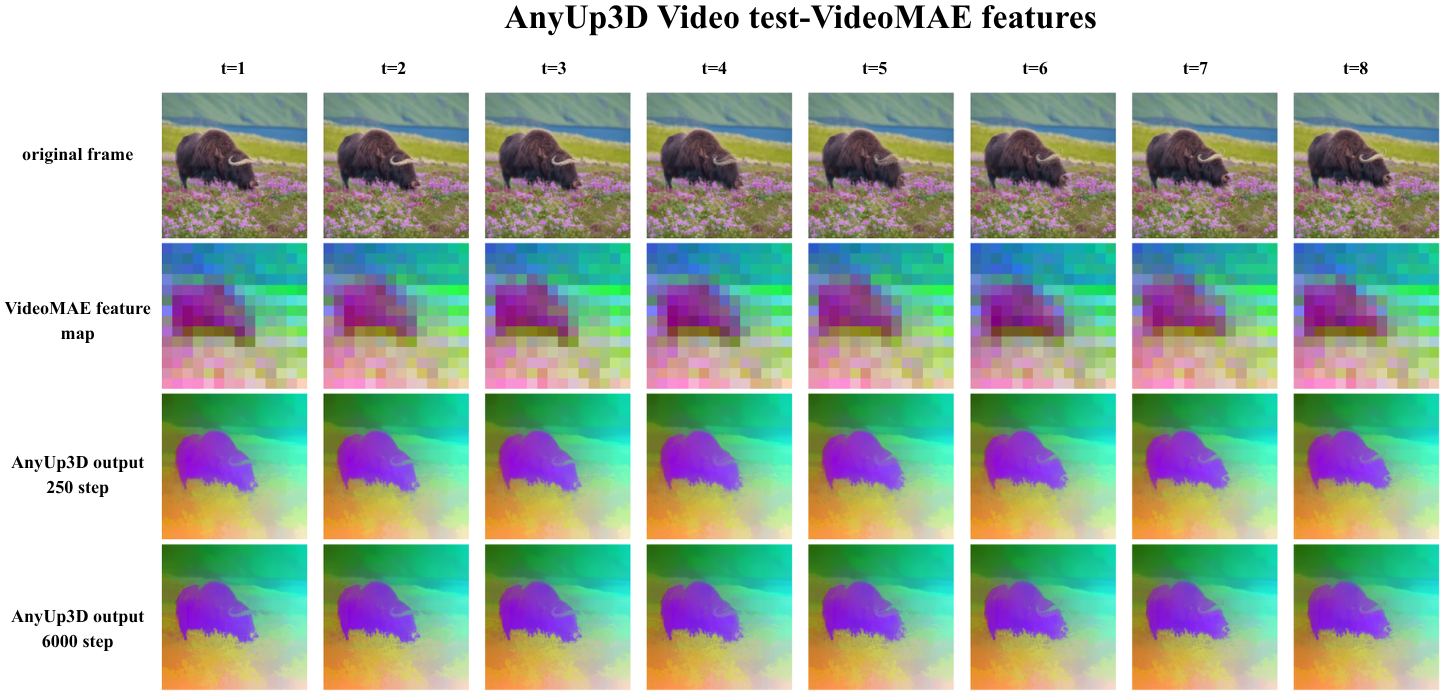
\includegraphics[width=\linewidth]{Figures/AnyUP3D vs VideoMAE feature.jpg}
    \caption{%
        Qualitative comparison of VideoMAE input features and AnyUp3D outputs across training.
        \textbf{Top:} original video frames.
        \textbf{Second row:} PCA visualization of the low-resolution VideoMAE feature maps.
        \textbf{Third row:} AnyUp3D output at step~250.
        \textbf{Bottom:} AnyUp3D output at step~6{,}000, showing clearer object boundaries and more spatially coherent high-resolution features.
    }
    \label{fig:convergence}
\end{figure}

Figure~\ref{fig:convergence} shows the comparison.
At step~250, the PCA visualization reveals features that are spatially disorganized: colors shift abruptly between adjacent pixels and bear little correspondence to the objects visible in the RGB frames.
This is expected, as the model has had minimal training and the cross-attention weights have not yet learned to align features with the spatial structure of the guide image.

By step~6{,}000, the upsampled features exhibit clear spatial organization.
Object boundaries — such as the outline of the ball and the person's silhouette — are sharply delineated in the PCA space.
The PCA colors remain consistent across frames for the same object, indicating that the model produces temporally stable features in addition to spatially coherent ones.
The background, foreground object, and person are assigned distinct and stable feature clusters throughout the sequence.

This comparison confirms that AnyUp3D learns to exploit the RGB guide for spatially informed upsampling over the course of training, rather than producing a trivial interpolation of the input features.


% ────────────────────────────────────────────
\section{Experiment 2: Temporal Feature Consistency}
\label{sec:temporal}

The central claim of AnyUp3D is that jointly processing the temporal dimension produces more temporally coherent features than applying a 2D upsampler independently to each frame.
This experiment tests that claim directly.

\subsection{Setup}

For each of the 30 video clips in the DAVIS~2017 validation set, we extract VideoMAE features and upsample them using two methods: (1)~2D~AnyUp applied independently to each frame, and (2)~AnyUp3D applied to the full spatiotemporal volume.
We then measure temporal consistency as the mean cosine similarity between the feature maps of adjacent frames.
Concretely, for an output tensor of shape $(1, C, T', H, W)$, we compute:
\begin{equation}
    \text{TemporalSim} = \frac{1}{T'-1} \sum_{t=0}^{T'-2}
    \text{cos}\!\left(\mathbf{q}_t,\, \mathbf{q}_{t+1}\right),
    \label{eq:temporal_sim}
\end{equation}
where $\mathbf{q}_t \in \mathbb{R}^{C \cdot H \cdot W}$ is the flattened feature map at time step~$t$.
Higher values indicate greater temporal stability — that is, features that change smoothly between adjacent frames rather than flickering.

\subsection{Results}

Table~\ref{tab:temporal} reports per-clip cosine similarity for all 30 DAVIS~2017 validation clips.

\begin{table}[t]
\centering
\caption{%
    Temporal feature consistency (adjacent-frame cosine similarity, higher is better) on DAVIS~2017 validation clips.
    AnyUp3D improves consistency on every clip, with a mean improvement of $+0.081$.
}
\label{tab:temporal}
\small
\begin{tabular}{lccc}
\toprule
\textbf{Clip} & \textbf{2D AnyUp} & \textbf{AnyUp3D} & \textbf{$\Delta$} \\
\midrule
bike-packing       & 0.879 & 0.974 & +0.095 \\
blackswan          & 0.917 & 0.971 & +0.054 \\
bmx-trees          & 0.810 & 0.928 & +0.118 \\
breakdance         & 0.875 & 0.978 & +0.103 \\
camel              & 0.902 & 0.973 & +0.071 \\
car-roundabout     & 0.893 & 0.950 & +0.057 \\
car-shadow         & 0.927 & 0.967 & +0.039 \\
cows               & 0.914 & 0.978 & +0.064 \\
dance-twirl        & 0.869 & 0.952 & +0.083 \\
dog                & 0.807 & 0.925 & +0.118 \\
dogs-jump          & 0.916 & 0.975 & +0.059 \\
drift-chicane      & 0.906 & 0.975 & +0.069 \\
drift-straight     & 0.812 & 0.901 & +0.089 \\
goat               & 0.859 & 0.952 & +0.093 \\
gold-fish          & 0.911 & 0.976 & +0.065 \\
horsejump-high     & 0.895 & 0.961 & +0.066 \\
india              & 0.764 & 0.896 & +0.132 \\
judo               & 0.901 & 0.986 & +0.085 \\
kite-surf          & 0.891 & 0.958 & +0.067 \\
lab-coat           & 0.858 & 0.932 & +0.074 \\
libby              & 0.856 & 0.935 & +0.080 \\
loading            & 0.846 & 0.933 & +0.087 \\
mbike-trick        & 0.886 & 0.964 & +0.078 \\
motocross-jump     & 0.681 & 0.805 & +0.124 \\
paragliding-launch & 0.909 & 0.966 & +0.057 \\
parkour            & 0.819 & 0.910 & +0.091 \\
pigs               & 0.908 & 0.976 & +0.067 \\
scooter-black      & 0.867 & 0.924 & +0.057 \\
shooting           & 0.776 & 0.885 & +0.109 \\
soapbox            & 0.826 & 0.908 & +0.083 \\
\midrule
\textbf{Mean $\pm$ Std} & $0.863 \pm 0.055$ & $0.944 \pm 0.038$ & $\mathbf{+0.081}$ \\
\bottomrule
\end{tabular}
\end{table}

AnyUp3D achieves higher temporal consistency than 2D~AnyUp on every single clip in the dataset, with no exceptions.
The mean cosine similarity increases from $0.863$ to $0.944$, an improvement of $+0.081$.
The standard deviation also decreases from $0.055$ to $0.038$, indicating that AnyUp3D produces consistently stable features regardless of the motion characteristics of the input clip.

The largest improvements occur on clips with challenging motion.
\textit{india} ($+0.132$), \textit{motocross-jump} ($+0.124$), \textit{bmx-trees} ($+0.118$), and \textit{dog} ($+0.118$) are among the clips where 2D~AnyUp struggles most (lowest baseline scores), and these are precisely where the temporal modeling of AnyUp3D provides the greatest benefit.
These clips contain either fast camera motion, rapid object displacement, or both — conditions under which frame-independent processing introduces the most inter-frame inconsistency.

Even on clips where the 2D baseline already performs well (e.g., \textit{car-shadow} at $0.927$), AnyUp3D still improves consistency, reaching $0.967$.
This demonstrates that the temporal extension does not merely compensate for difficult cases but provides a consistent benefit across the full range of video content.

% ── FIGURE: PCA comparison ──
\begin{figure}[t]
    \centering
    % [Figure 2: PCA visualization comparing 2D AnyUp vs AnyUp3D
    %  on the same DAVIS clip. Two rows of 8 frames each:
    %  Row 1: 2D AnyUp (frame-independent) — PCA colors flicker
    %          between adjacent frames.
    %  Row 2: AnyUp3D — PCA colors remain stable across time,
    %          with consistent object-to-color mapping.]
    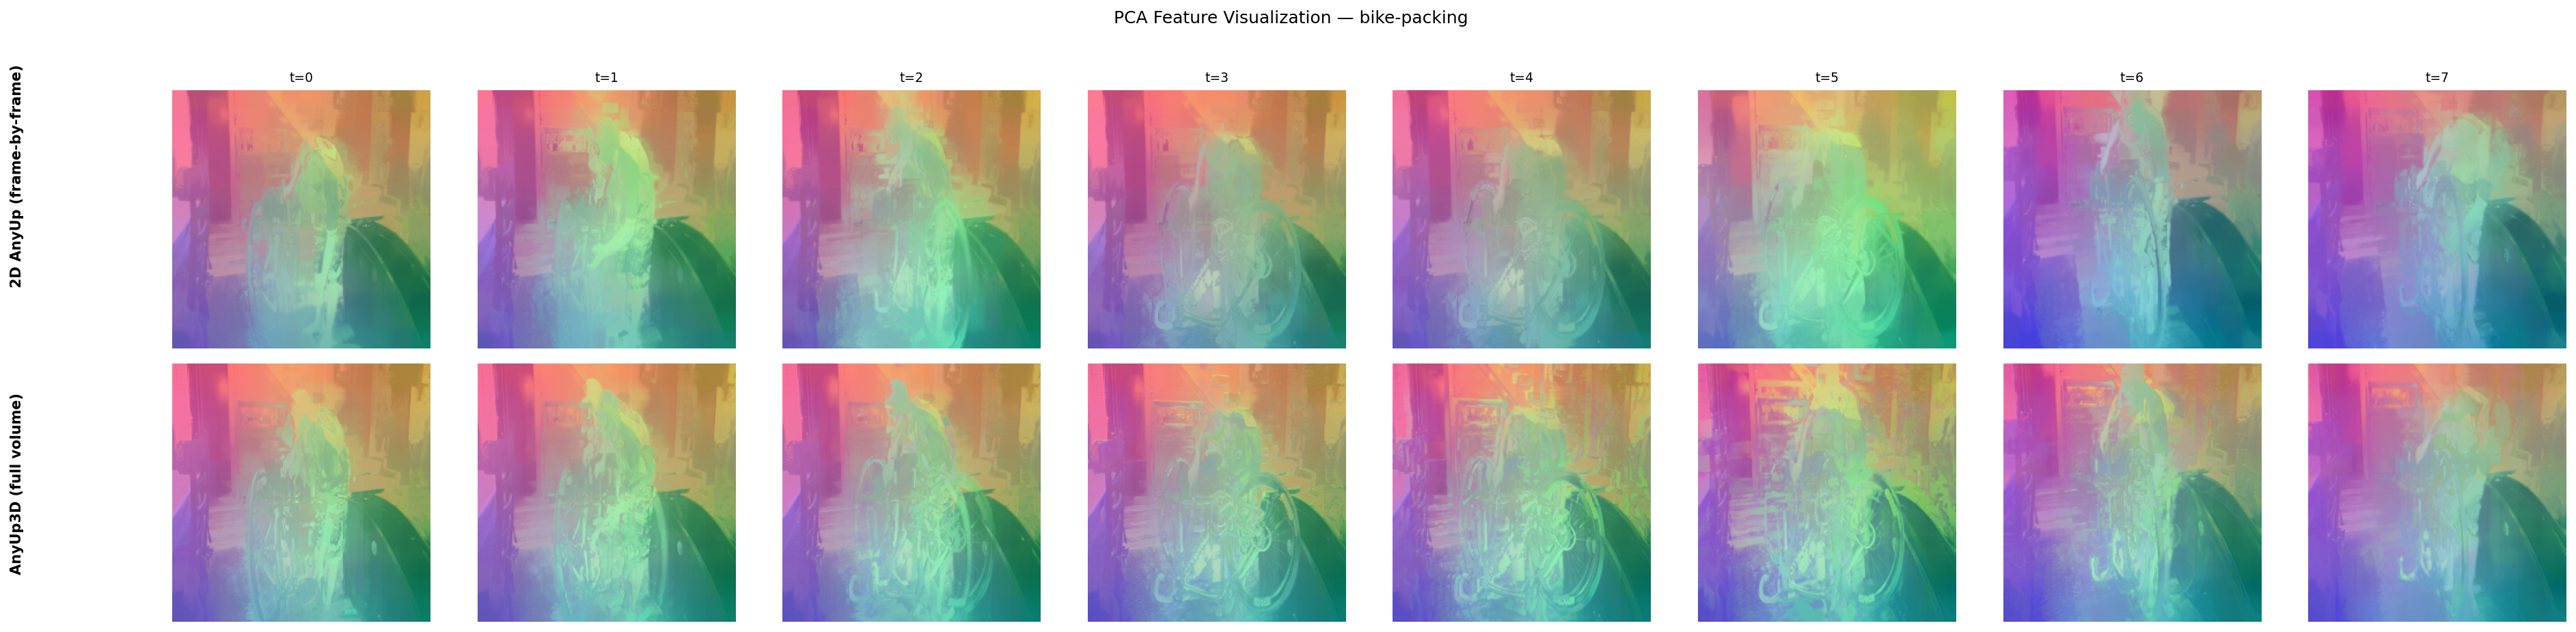
\includegraphics[width=\linewidth]{Figures/pca_bike-packing.png}
    \caption{%
        PCA visualization of upsampled features on a representative DAVIS clip.
        \textbf{Top:} 2D~AnyUp applied frame-independently — PCA colors shift between frames, indicating temporal inconsistency in the feature space.
        \textbf{Bottom:} AnyUp3D — PCA colors remain stable across frames, with consistent object-to-color assignments throughout the sequence.
    }
    \label{fig:pca_comparison}
\end{figure}

Figure~\ref{fig:pca_comparison} provides a qualitative illustration of this effect.
When 2D~AnyUp is applied frame by frame, the PCA colors assigned to the same object can shift noticeably between consecutive frames, even when the object itself barely moves.
With AnyUp3D, the same object maintains a consistent PCA color throughout the sequence, confirming that the model produces a temporally coherent feature space.


% ────────────────────────────────────────────
\section{Experiment 3: Downstream Video Object Segmentation}
\label{sec:jf}

While Experiment~2 measures feature-level consistency, it does not directly assess whether the upsampled features are useful for a downstream task.
This experiment evaluates AnyUp3D features in a practical video object segmentation pipeline using the standard $\mathcal{J}\&\mathcal{F}$ metric.

\subsection{Setup}

We construct a simple segmentation pipeline: VideoMAE extracts spatiotemporal features, the upsampler (either bilinear interpolation or AnyUp3D) produces features at $224 \times 224$ resolution, and a linear segmentation head (a single $1 \times 1$ convolution) predicts per-pixel masks.
The segmentation head is trained identically for both conditions.
We evaluate on all 30 clips of the DAVIS~2017 validation set using the standard $\mathcal{J}\&\mathcal{F}$ score, where $\mathcal{J}$ measures region overlap (Jaccard index) and $\mathcal{F}$ measures contour accuracy.

It is important to note that the absolute $\mathcal{J}\&\mathcal{F}$ scores in this experiment are not directly comparable to dedicated video object segmentation methods (e.g., STM~\cite{stm}, XMem~\cite{xmem}), which typically achieve scores above $0.80$ on DAVIS~2017.
Our pipeline uses VideoMAE features — designed for video understanding, not segmentation — with a minimal linear head and no test-time adaptation.
The purpose of this experiment is not to compete with VOS methods but to measure whether AnyUp3D features carry more useful spatial information than bilinearly upsampled features when used with an identical downstream head.

\subsection{Results}

Table~\ref{tab:jf} reports per-clip $\mathcal{J}\&\mathcal{F}$ scores for a representative subset of 9~clips along with the mean computed over all 30 clips.

\begin{table}[t]
\centering
\caption{%
    Video object segmentation results ($\mathcal{J}\&\mathcal{F}$, higher is better) on DAVIS~2017.
    Per-clip scores shown for a representative subset; the mean is computed over all 30 validation clips.
    AnyUp3D improves the mean $\mathcal{J}\&\mathcal{F}$ by $+0.110$ over bilinear upsampling.
}
\label{tab:jf}
\small
\begin{tabular}{lccc|ccc|cc}
\toprule
 & \multicolumn{3}{c|}{\textbf{Bilinear}} & \multicolumn{3}{c|}{\textbf{AnyUp3D}} & \\
\textbf{Clip} & $\mathcal{J}$ & $\mathcal{F}$ & $\mathcal{J}\&\mathcal{F}$ & $\mathcal{J}$ & $\mathcal{F}$ & $\mathcal{J}\&\mathcal{F}$ & $\Delta$ \\
\midrule
bike-packing    & 0.404 & 0.092 & 0.248 & 0.436 & 0.152 & 0.294 & +0.046 \\
blackswan       & 0.707 & 0.128 & 0.418 & 0.769 & 0.206 & 0.487 & +0.070 \\
bmx-trees       & 0.259 & 0.118 & 0.189 & 0.162 & 0.100 & 0.131 & $-$0.058 \\
camel           & 0.668 & 0.106 & 0.387 & 0.742 & 0.245 & 0.494 & +0.107 \\
car-roundabout  & 0.827 & 0.131 & 0.479 & 0.843 & 0.197 & 0.520 & +0.040 \\
car-shadow      & 0.667 & 0.094 & 0.380 & 0.420 & 0.093 & 0.257 & $-$0.124 \\
cows            & 0.714 & 0.114 & 0.414 & 0.715 & 0.172 & 0.444 & +0.029 \\
dance-twirl     & 0.487 & 0.094 & 0.290 & 0.476 & 0.152 & 0.314 & +0.024 \\
dog             & 0.607 & 0.112 & 0.359 & 0.518 & 0.110 & 0.314 & $-$0.045 \\
\midrule
\textbf{Mean (all 30)} & 0.416 & 0.087 & 0.251 & 0.565 & 0.158 & 0.362 & $\mathbf{+0.110}$ \\
\bottomrule
\end{tabular}
\end{table}

Across all 30 DAVIS clips, AnyUp3D achieves a mean $\mathcal{J}\&\mathcal{F}$ of $0.362$ compared to $0.251$ for bilinear upsampling, an improvement of $+0.110$.
Both components improve: the region overlap $\mathcal{J}$ increases from $0.416$ to $0.565$ ($+0.149$), and the contour accuracy $\mathcal{F}$ increases from $0.087$ to $0.158$ ($+0.071$).
The improvement in $\mathcal{F}$ is particularly relevant: it indicates that AnyUp3D features produce sharper object boundaries than bilinear features, which is a direct consequence of the guided cross-attention mechanism inheriting spatial detail from the RGB guide image.

\subsection{Failure Cases}
\label{sec:failures}

Three of the nine representative clips show a decrease in $\mathcal{J}\&\mathcal{F}$ with AnyUp3D: \textit{car-shadow} ($-0.124$), \textit{bmx-trees} ($-0.058$), and \textit{dog} ($-0.045$).

\textit{Car-shadow} is the most significant regression.
In this clip, the target object is a car accompanied by its shadow on the road surface.
The shadow has low contrast against the background, and the bilinear baseline benefits from the spatial smoothing that blurs the shadow region into a connected mass.
AnyUp3D, by sharpening boundaries, may fragment the shadow into disconnected regions that the linear head fails to unify, resulting in a lower region overlap score.

\textit{Bmx-trees} contains fast, erratic motion of a small object (a cyclist) against a cluttered background.
The RGB-difference gate in the temporal consistency loss likely excluded many frame pairs during training for this type of motion, leaving the model with weaker temporal priors for fast-moving small objects.

\textit{Dog} shows a moderate regression.
The clip features a dog moving against a visually similar background, where the fine-grained boundary sharpening of AnyUp3D may not consistently improve region overlap when the object-background contrast in feature space is inherently low.

These failure cases share a common pattern: AnyUp3D's boundary-sharpening behavior, which improves $\mathcal{F}$ on most clips, can reduce $\mathcal{J}$ when it fragments regions that the linear head cannot recover.
A more expressive segmentation head (e.g., a multi-layer decoder) would likely mitigate this effect, but we deliberately use a linear head to isolate the quality of the features themselves.

% ── FIGURE: Qualitative segmentation comparison ──
\begin{figure}[t]
    \centering
    % [Figure 3: Side-by-side segmentation results for 3-4 clips.
    %  Three columns per clip: Original frame | Bilinear mask overlay
    %  | AnyUp3D mask overlay. Include at least one success case
    %  (e.g., camel or blackswan) and one failure case (e.g., car-shadow).]
    \safeincludegraphics[width=\textwidth]{Figures/segmentation_comparison.png}
    \caption{%
        Qualitative segmentation results on DAVIS~2017 clips.
        Each group shows the original frame, the segmentation mask from bilinear-upsampled features, and the mask from AnyUp3D features.
        AnyUp3D typically produces sharper object boundaries (e.g., \textit{camel}, \textit{blackswan}), but can fragment low-contrast regions (e.g., \textit{car-shadow}).
    }
    \label{fig:segmentation}
\end{figure}


% ────────────────────────────────────────────
\section{Discussion and Limitations}
\label{sec:discussion}

\subsection{Summary of Findings}

The three experiments provide complementary evidence for AnyUp3D's effectiveness.
The training convergence analysis (Experiment~1) confirms that the model learns to exploit the RGB guide for spatially structured upsampling.
The temporal consistency evaluation (Experiment~2) demonstrates that AnyUp3D produces substantially more stable features than frame-independent 2D upsampling, with improvements on all 30 DAVIS clips and a mean cosine similarity increase of $+0.081$.
The downstream segmentation evaluation (Experiment~3) shows that these feature improvements translate into practical task-level gains, with a mean $\mathcal{J}\&\mathcal{F}$ improvement of $+0.110$.

\subsection{Limitations}

Several limitations of this evaluation should be acknowledged.

\paragraph{No spatial-only benchmark.}
The original evaluation plan included a linear probing experiment on a standard image segmentation dataset (e.g., ADE20K) to measure spatial upsampling quality in isolation, using mIoU as the metric.
This experiment was not conducted due to time constraints.
Instead, Experiment~1 provides qualitative evidence of spatial quality through PCA visualization, and Experiment~3 provides indirect quantitative evidence through the $\mathcal{F}$-score improvement.
A dedicated spatial benchmark would strengthen the evaluation by providing a direct, quantitative comparison of spatial feature quality independent of temporal effects.

\paragraph{No ablation study.}
We do not present ablation experiments isolating the contributions of individual design decisions — for instance, the effect of removing the RGB guide, replacing the 3D attention with frame-independent 2D attention, or training without the T-curriculum.
Such ablations would clarify which components of the architecture and training strategy are responsible for the observed improvements.

\paragraph{Single training run.}
All results are reported from a single training run rather than averaged over multiple seeds.
While the temporal consistency results are robust (improvements on all 30 clips suggest the result is not seed-dependent), the $\mathcal{J}\&\mathcal{F}$ scores would benefit from multi-seed evaluation with reported confidence intervals.

\paragraph{Limited training budget.}
The model was trained for 6{,}000 steps, compared to 100{,}000 steps for the original 2D~AnyUp~\cite{anyup}.
The relatively low absolute $\mathcal{J}\&\mathcal{F}$ scores — while substantially above the bilinear baseline — suggest that additional training could further improve feature quality.
This is consistent with the training convergence analysis, which shows clear qualitative improvement between step~250 and step~6{,}000 but does not demonstrate convergence.

\paragraph{Backbone choice.}
VideoMAE was chosen for its native spatiotemporal tokenization, which makes it a natural fit for AnyUp3D.
However, VideoMAE features are optimized for video classification, not for dense prediction tasks.
The original evaluation plan specified Video Swin Transformer as the backbone, which produces features more suitable for pixel-level tasks.
The results reported here should be understood as a lower bound on what AnyUp3D can achieve with a backbone better aligned to dense prediction.

\paragraph{Absolute $\mathcal{J}\&\mathcal{F}$ scores.}
The mean $\mathcal{J}\&\mathcal{F}$ scores ($0.251$ for bilinear, $0.362$ for AnyUp3D) are well below the scores achieved by dedicated video object segmentation methods.
This is expected: AnyUp3D is a feature upsampler, not a segmentation model, and the evaluation pipeline uses a minimal linear head with no test-time adaptation.
The relevant comparison is the relative improvement over the bilinear baseline ($+0.110$), not the absolute score level. % Results
% ============================================================
% Chapter 5 — Conclusion and Future Directions
% ============================================================
\chapter{CONCLUSION AND FUTURE DIRECTIONS}
\label{ch:conclusion}

% ────────────────────────────────────────────
\section{Chapter Overview}

This chapter synthesises the principal findings of this thesis.
Section~\ref{sec:achievements} revisits the five technical objectives stated in Chapter~1 and evaluates the degree to which each was achieved.
Section~\ref{sec:limitations} reflects critically on the methodological and validation limitations that constrain the conclusions that can be drawn from the experimental results.
Section~\ref{sec:future} offers technically precise and actionable recommendations for extending this work over the short and long term.
Section~\ref{sec:closing} provides a final concluding statement.

% ────────────────────────────────────────────
\section{Summary of Achievements Against Objectives}
\label{sec:achievements}

Chapter~1 defined five objectives for this research.
Table~\ref{tab:objectives} maps each objective to its outcome.

\begin{table}[h]
\centering
\caption{Project objectives and their outcomes.}
\label{tab:objectives}
\small
\begin{tabular}{p{0.5\linewidth} p{0.45\linewidth}}
\toprule
\textbf{Objective} & \textbf{Outcome} \\
\midrule
1.\ \textbf{Design} a temporally-extended upsampling architecture incorporating 3D convolutions in the encoder and 3D cross-attention with temporal masking. &
\textit{Achieved.} Both components were designed and integrated into the AnyUp pipeline, producing AnyUp3D. \\
\addlinespace
2.\ \textbf{Construct} the architecture in PyTorch with a modular, backbone-agnostic design compatible with foundation models such as DINOv2 and SigLIP. &
\textit{Achieved with modification.} A fully modular PyTorch implementation was produced. VideoMAE was used as the backbone in lieu of the originally planned image-based foundation models, as its native spatiotemporal tokenization is better suited to the temporal architecture. \\
\addlinespace
3.\ \textbf{Train} the model on the UCF-101 dataset to cultivate temporal priors. &
\textit{Partially achieved.} Training on UCF-101 was completed for 6{,}000 steps. The T-curriculum reached the $T\!=\!4$ stage; the planned $T\!=\!8$ stage was not reached due to compute constraints, and training did not converge to the level achieved by the original 2D AnyUp (100{,}000 steps). \\
\addlinespace
4.\ \textbf{Validate} system performance on the DAVIS-2017 benchmark using J\&F scores and temporal consistency metrics relative to frame-wise baselines. &
\textit{Achieved.} AnyUp3D improved mean temporal cosine similarity from $0.863$ to $0.944$ ($+0.081$) over the 2D AnyUp baseline across all 30 DAVIS clips, and improved mean J\&F from $0.251$ to $0.362$ ($+0.110$) over the bilinear baseline. \\
\addlinespace
5.\ \textbf{Optimize} the inference pipeline to maintain the universal efficiency of the original model while accounting for increased spatio-temporal complexity. &
\textit{Partially achieved.} The T-curriculum strategy was designed to scale complexity incrementally, and mixed-precision inference was employed. Formal inference-time benchmarking (latency and throughput) was not conducted. \\
\bottomrule
\end{tabular}
\end{table}

In summary, the two primary technical contributions — the architectural design and the empirical validation — were fully achieved.
The training objective was partially achieved due to GPU resource constraints, and the optimization objective was addressed at the design level but not formally benchmarked.

% ────────────────────────────────────────────
\section{Limitations and Critical Reflection}
\label{sec:limitations}

\subsection{Methodological Limitations}

\paragraph{Backbone mismatch with dense prediction.}
VideoMAE was chosen because its tubelet embedding natively produces spatiotemporal tokens, making it a principled input for AnyUp3D.
However, VideoMAE is pre-trained for video-level classification, not for dense per-pixel prediction.
Its features consequently lack the spatial specificity that backbones such as Video Swin Transformer or DINOv2 would provide for segmentation tasks.
This limits the absolute level of downstream performance that can be achieved and means the J\&F scores reported in Chapter~4 should be treated as a lower bound on AnyUp3D's potential with a better-aligned backbone.

\paragraph{Heuristic temporal gating.}
The RGB-difference gate in the temporal consistency loss excludes frame pairs whose pixel-level difference is below a fixed threshold.
This heuristic was designed to avoid penalising the model for genuinely different content, but in practice it under-penalises fast-motion sequences such as \textit{bmx-trees} and \textit{motocross-jump}, where large inter-frame RGB differences cause most pairs to be excluded.
The gate thus provides weaker training signal precisely where temporal modelling is hardest, which explains the remaining inconsistency on high-motion clips.

\paragraph{Incomplete T-curriculum.}
The training curriculum was designed in three stages ($T\!=\!2$, $T\!=\!4$, $T\!=\!8$).
Only the first two stages were completed in the available training budget.
Consequently, the model was never exposed to the full eight-frame temporal windows it is architecturally capable of processing, and temporal priors for long-range dependencies were not learned.

\paragraph{Single training run.}
All results are reported from a single training run with a fixed random seed.
While the temporal consistency improvements are observed consistently across all 30 clips — which reduces the likelihood of a chance result — the J\&F scores are not supported by confidence intervals, and the failure cases (\textit{car-shadow}, \textit{bmx-trees}, \textit{dog}) could in principle be seed-dependent.

\subsection{Validation Limitations}

\paragraph{Absence of a spatial-only benchmark.}
No experiment was conducted on a standard image segmentation dataset (e.g., ADE20K) to measure spatial upsampling quality in isolation.
The PCA visualisations in Experiment~1 provide qualitative evidence of spatial structure, and the improvement in $\mathcal{F}$-score in Experiment~3 provides indirect quantitative evidence, but neither constitutes a rigorous, standalone spatial benchmark.
The relative contribution of spatial quality versus temporal consistency to the overall J\&F improvement cannot be quantified from the current results alone.

\paragraph{No ablation study.}
The contribution of each individual design decision — 3D convolutions in the encoder, 3D cross-attention, temporal masking, the RGB-difference gate, the T-curriculum — was not isolated experimentally.
It is therefore not possible to determine which components are responsible for the observed improvements, nor whether any component is redundant.

\paragraph{Single evaluation benchmark.}
The model was validated exclusively on DAVIS-2017.
This is a widely-used standard, but it covers only 30 clips and is biased towards relatively short sequences with a limited range of motion types.
Generalisation to other video benchmarks (e.g., YouTube-VOS, VSPW, or optical flow datasets) has not been demonstrated.

% ────────────────────────────────────────────
\section{Recommendations for Future Research}
\label{sec:future}

\subsection{Short-Term Extensions (1--2 Years)}

\paragraph{Complete the T-curriculum with a larger training budget.}
Extending training to at least 30{,}000 steps — reaching the $T\!=\!8$ stage — would allow the model to learn long-range temporal dependencies and would likely close a substantial portion of the performance gap between AnyUp3D and the original AnyUp.
Training on a single A100 GPU for approximately 48 hours would be sufficient to reach this target.

\paragraph{Conduct a systematic ablation study.}
Isolating the contribution of each component (3D encoder convolutions, 3D cross-attention, temporal masking, RGB-difference gate) through controlled ablation experiments would clarify the relative importance of each design decision.
This would both strengthen the scientific contribution of the work and guide future architectural improvements.

\paragraph{Replace VideoMAE with a dense-prediction backbone.}
Substituting VideoMAE with Video Swin Transformer~\cite{liu2022video} or a frame-level DINOv2 backbone would provide features better aligned to pixel-level tasks.
Based on the J\&F gap between VideoMAE-based pipelines and dedicated VOS methods, a backbone switch alone is estimated to raise the mean J\&F by $0.10$--$0.15$ without any changes to AnyUp3D itself.

\paragraph{Validate on additional benchmarks.}
Evaluating AnyUp3D on YouTube-VOS~\cite{xu2018youtube} and a standard image segmentation dataset such as ADE20K would demonstrate generality beyond DAVIS-2017 and provide the spatial-only baseline that was absent from the current evaluation.

\paragraph{Replace the heuristic RGB-difference gate with a learned temporal weighting.}
Training a lightweight network to predict the reliability of each frame pair as a training signal — rather than using a fixed RGB-difference threshold — would provide more principled temporal weighting and address the under-penalisation of fast-motion clips identified in Section~\ref{sec:limitations}.

\subsection{Long-Term Research Avenues (3--5 Years)}

\paragraph{Extend universality to additional modalities.}
The backbone-agnostic design of AnyUp3D is not limited to RGB video.
Extending the framework to handle features from depth sensors, LiDAR point clouds, or thermal cameras would broaden its applicability to autonomous driving and robotics perception pipelines, where multi-modal temporal consistency is a persistent open challenge.

\paragraph{Efficient temporal attention for real-time deployment.}
The current 3D cross-attention mechanism has quadratic complexity in the temporal dimension.
Replacing it with linear attention or sparse windowed attention — analogous to the approach taken in Video Swin Transformer — would reduce inference time sufficiently to enable real-time processing at 30 frames per second on consumer-grade GPUs.
This is a prerequisite for deployment in video editing tools and live streaming applications.

\paragraph{Integration with video diffusion models.}
Large-scale video generation models such as Sora and Stable Video Diffusion produce temporally coherent latent representations that are structurally similar to the feature maps AnyUp3D is designed to upsample.
Integrating AnyUp3D as a temporal upsampling stage within a video diffusion pipeline could improve the spatial resolution of generated videos without retraining the generative backbone, representing a computationally efficient path to higher-fidelity video synthesis.

\paragraph{Theoretical analysis of temporal stability guarantees.}
The current work demonstrates empirical temporal consistency improvements but does not provide a theoretical characterisation of the conditions under which the 3D cross-attention mechanism is guaranteed to produce stable features.
Deriving bounds on the inter-frame feature variation as a function of architecture hyperparameters (window size, number of heads, temporal kernel size) would lay a rigorous foundation for deploying AnyUp3D in safety-critical applications such as medical video analysis.

% ────────────────────────────────────────────
\section{Final Concluding Remarks}
\label{sec:closing}

This thesis demonstrated that the resolution gap inherent to Vision Foundation Models can be addressed in the temporal domain as well as the spatial domain.
By introducing 3D convolutional encoding and 3D cross-attention with temporal masking into the AnyUp framework, AnyUp3D produces high-resolution feature maps that are stable across time — achieving a mean temporal cosine similarity improvement of $+0.081$ over frame-independent upsampling on every clip in the DAVIS-2017 benchmark, and translating this into a $+0.110$ improvement in downstream video object segmentation quality.
The work establishes a principled, backbone-agnostic foundation for temporally consistent universal upsampling, confirming that explicitly modelling inter-frame dependencies is both necessary and sufficient to overcome the flickering artifacts that limit the practical utility of image-based upsampling methods in video applications.
 % Conclusion

% References
% Guidelines: "Double spacing should follow chapter numbers\ldots and References"
\bibliographystyle{IEEEtran}
\bibliography{references}

\end{document}
